\chapter{Autonomous Cars Localization for GPS-denied Urban Environments}

\section{Introduction}


\section{Localization Based on Satellite Aerial Maps}

Figure 1 presents an overview of the proposed system architecture. Our system is divided into two main components: offline and online parts. The offline part is responsible for creating a large grey-scale map image of the region of interest. This is achieved by downloading individual aerial pictures and stitching them together.

The online part implements a Particle Filter Localization (PFL) algorithm [15]. The PFL system is initialized by sampling the particles on top of the aerial image map according to the first GPS and compass readings. During the prediction phase, the PFL considers the vehicle's movement disturbed by a Gaussian noise to cover the real positions as hypotheses. Thereafter, the LiDAR is used to create a local re-emission map, which is built using the infrared reflectance of the Velodyne's lasers together with the returned distance information and dead-reckoning. This re-emission map is accumulated for a few time steps and it is compared against the aerial map in order to estimate the particles' weights. The comparison is performed using NMI. Based on the weights, the best particles are selected to calculate the global pose according to the weighted average of their position. Please note that the information from the GPS and the compass are used only to globally initialize the PFL algorithm.

\subsection{Offiline Aerial Map}

A large aerial image for the region of interest is created by first downloading individual images with a $640\times640$ pixel resolution. Individual images overlap each other and the overlapping region is used to calculate the correspondences between them that are necessary for image registration and stitching. This step is performed once manually using the Microsoft ICE software. Unfortunately, the minimum grid-size (zoom level) of the region of interest is close to 0.29 meters. In order to avoid rounding problems, we rescaled the stitched map to 0.2 meters. Figure \ref{Fig::Path} shows the car's route and aerial images of challenging environments where the car was driven and localized (red line).

\begin{figure}[ht]
    \centering
    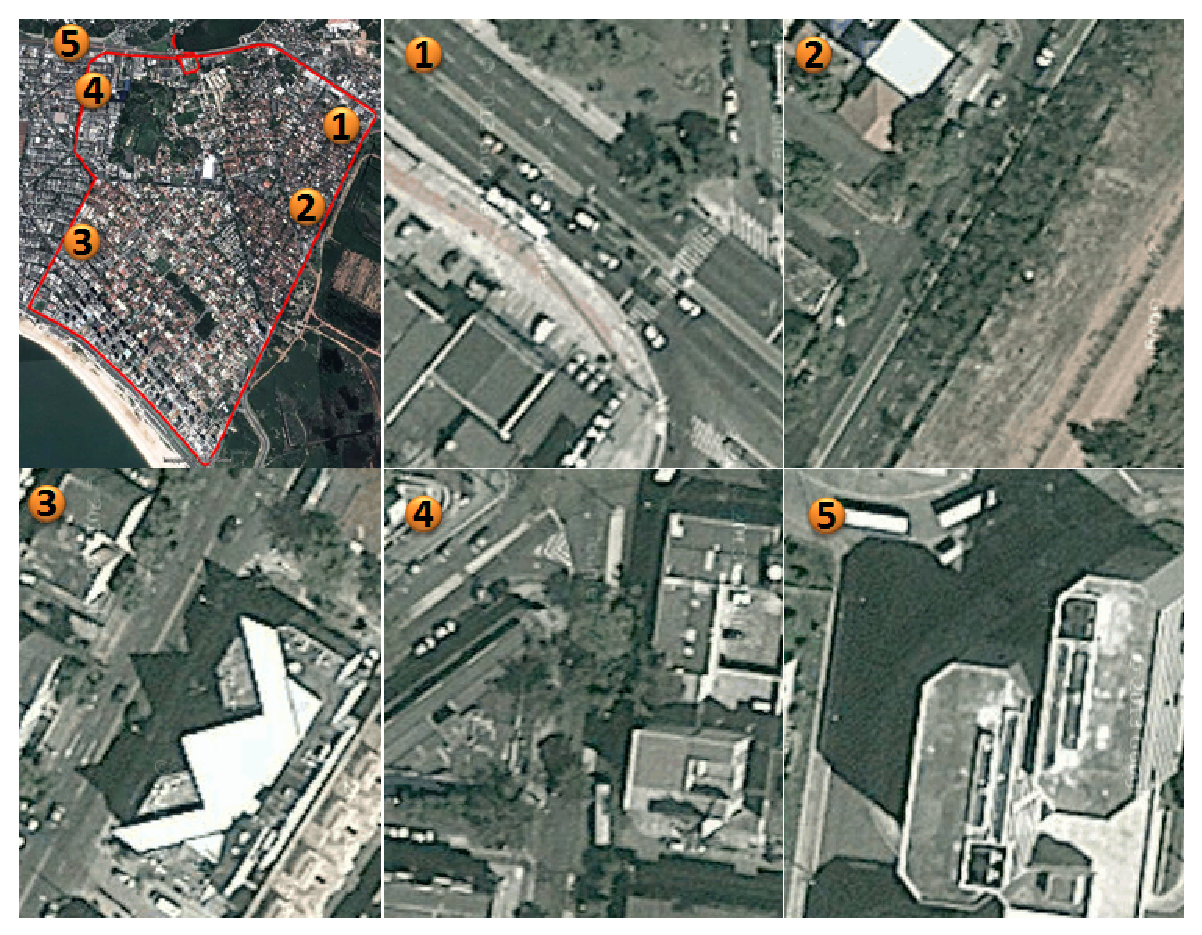
\includegraphics[width = 100 mm]{path.eps}
    \caption{Satellite map images used to localize the robot in a large urban area. The red line on the top-left image represents the car's route. The other images (1-5) are zoom up examples of aerial image maps used by our approach to localize the vehicle.}
    \label{Fig::Path}
\end{figure}

\subsection{Online Re-emission Grid-Map}

An online short-term re-emission grid-map (a local top view image) is built with $60\times60$ meters and 0.2 meters of resolution per pixel. This grid-map is a gray-scale image (i.e., $[0, 255]$) produced by the projection of every laser in 2D (see Figure \ref{Fig::Remission1}). Every pixel, i.e. map cell, in the grid-map stores the average of the infrared reflectance of the rays which touched it. The map shows several features (such as curbs, lanes, sidewalks, asphalt, etc), which are important for feature-comparison in the localization process of the mobile robot. Note that the short-term map accumulates the information of several Velodyne's scans in an area of approximately 3600 $m^2$ and that the robot dead-reckoning is considered when posing the scans in the local map. Figure \ref{Fig::Remission1} shows the short-term map after some Velodyne's scans. In this figure, the blue parts are non-sensed areas in the environment, gray scale areas are the average of the infrared reflectance, and the orange rectangle illustrates the robot position. Note that non-sensed areas (i.e. blue areas) are not considered during the distance measurement computation.



\begin{figure}[ht]
    \centering
    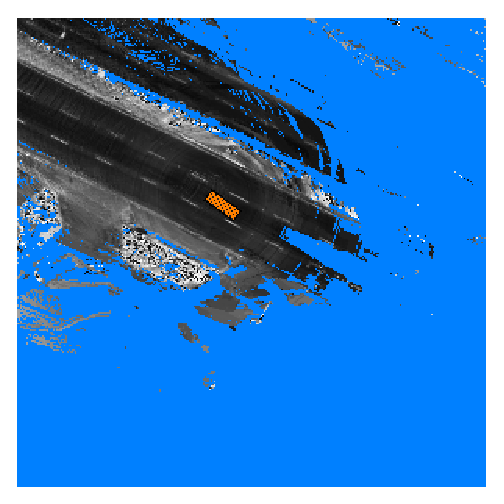
\includegraphics[width = 50 mm]{Remission1.eps}
    \caption{Local short-term re-emission grid-map with $60\times60$ meters built using the LiDAR. In this figure the blue parts are the non-sensed areas in the environment. Grey values indicate the average values of the laser infrared reflectance. The orange rectangle illustrates the robot position given by the dead-reckoning.}
    \label{Fig::Remission1}
\end{figure}

\subsection{Grid Map Construction and Representation}
\label{sec::ch2-mapping}

The mapping subsystem receives as input the Velodyne point clouds and its respective poses calculated by the dead-reckoning and outputs local grid maps.  In the grid maps, the environment is divided into cells with the same size (the size of the cells is usually called map resolution) and each of these cells contains some kind of local information about the environment.  There are several types of grid maps, e.g. occupancy grid maps, re-emission grid maps and likelihood-field grid maps. In occupancy grid maps, each cell contains the probability of the cell being occupied by an obstacle. In re-emission grid maps, each cell stores the average infrared reflectance of the rays that hit that cell \cite{13levinson2007map}.Thus, re-emission grid maps have the appearance of an image of the ground plane. Finally, in likelihood-field grid maps, each cell stores the Gaussian of the distance to the nearest obstacle \cite{26thrun2005probabilistic}.

To illustrate the described maps, \ref{Fig::FIGURE04A}, Figure \ref{Fig::FIGURE04B}, and Figure \ref{Fig::FIGURE04C} show occupancy grid map, re-emission grid map and likelihood-field grid map. All the maps have $60\times60$ meters and $0.2$ meters of map resolution. In Figure \ref{Fig::FIGURE04A}, the occupancy probability is represented in gray-scale where $255$ is the minimum probability of obstacles and $0$ is the maximum probability. The blue areas are unknown places in the environment. In Figure \ref{Fig::FIGURE04B}, the re-emission of the cells hit by the sensor rays are shown in gray and the blue area represents not hit cells. In Figure \ref{Fig::FIGURE04C}, the occupancy likelihood field is represented in gray-scale, where $255$ represents the lowest occupancy likelihood and $0$ represents the highest occupancy likelihood. The likelihood field model is an ``ad hoc'' alternative to the traditional beam model. While it lacks a plausible physical explanation, it provides important advantages, such as smoother posteriors even in cluttered spaces, and more efficient computation \cite{26thrun2005probabilistic}. In the likelihood field model, the probability of a sensor measurement is obtained by measuring the distance from the laser reading to the nearest obstacle in the map and applying this distance to a zero-centered Gaussian \cite{26thrun2005probabilistic}. Naturally, the probability is maximal when the distance is zero (the laser reading hit an obstacle in the map), and decreases as the distance get bigger. Because of this feature, areas of the map in which there are no information about obstacles (and it includes unseen areas), are filled with close to zero occupancy probabilities once their distance to the nearest obstacle are significantly bigger than zero. Even we emphasizing the development of occupancy grid maps, the LEMS can be adapted, with small modifications, to generate likelihood field-based (or any other kind of) grid maps.

\begin{figure}[t]
	\centering
	\subfloat[]{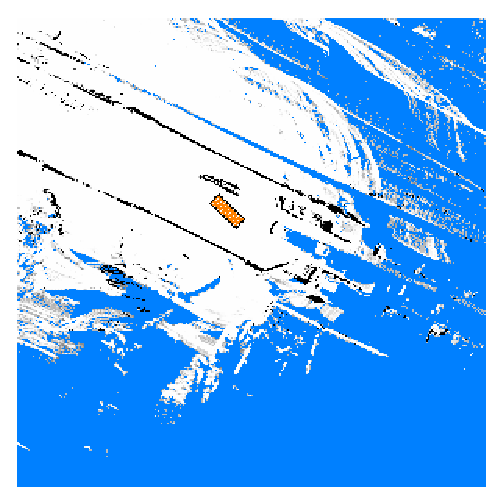
\includegraphics[width=42mm]{Occupancy1}
		\label{Fig::FIGURE04A}}
	\subfloat[]{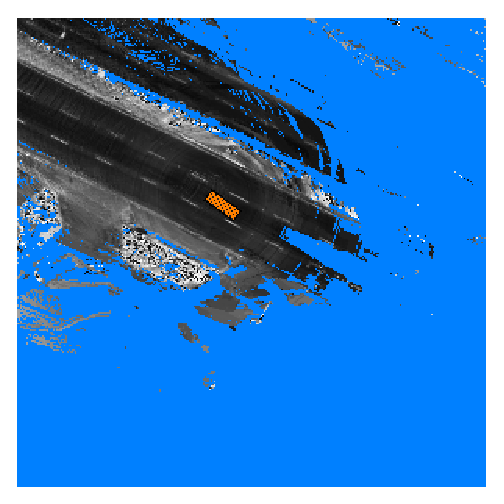
\includegraphics[width=42mm]{Remission1}
		\label{Fig::FIGURE04B}}\\
	\subfloat[]{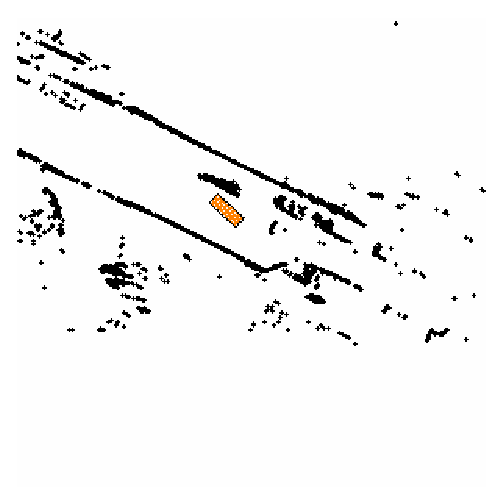
\includegraphics[width=42mm]{Occupancy3}
		\label{Fig::FIGURE04C}}
	\caption{Maps constructed by the Mapping process. (a) Occupancy grid map with $60\times60$ meters and 0.2 meters of resolution built using 3D LiDAR sensor projected to 2D. The blue parts are unknown places in the environment. (b) Re-emission grid map. (b) Likelihood-Field grid map.}
	\label{Fig::FIGURE04}
\end{figure}

The algorithm to build occupancy grid maps consists of initializing all cells with a neutral probability and then increasing or decreasing the cell occupancy probability depending if the laser ray hits an obstacle or a free area. The classical choices for the neutral probability are to use $0.5$ to represent that a cell has the same probability of being occupied or free, and to use an invalid value (e.g. $-1$) to represent that the cell occupancy probability is unknown. In this work, we used the second option. To avoid numerical inconsistency due to near to one or near to zero probabilities, we represent the occupancy probability using log-odds \cite{26thrun2005probabilistic}.

The data provided by the Velodyne sensor was used to update the occupancy probability of the map cells. The Velodyne consists of a set of vertical lasers that spins around the vertical axis in order to capture a 3D point cloud of the environment. As Velodyne provides point clouds in 3D spherical coordinates, it is necessary to project the rays to 2D to calculate the cells hit by the rays. Due to the particular structure of the sensor readings, we used a special method to detect if a laser ray hits an obstacle or a free area (the method is described in detail in the next subsection). Besides of updating the cells hit by the laser rays, we used a ray cast scheme to quickly mark the free areas close to the vehicle. This scheme consists of decreasing, for each set of vertical readings, the occupancy probability of the grid cells between the sensor and nearest detected obstacle.

\subsection{Obstacle Classification}

Here, we describe how to detect if a Velodyne ray hits an obstacle or a free area. Our obstacle detection technique assumes that the 3D point clouds are represented in spherical coordinates. We will use the notation $z_t^{i,j}$ to represent the $i^{th}$ ray of the $j^{th}$ vertical set of readings captured at instant t. To compute the obstacle evidence (OE) of the ray $z_t^{i+1,j}$, its size projected on the ground is compared with the size of the previous ray $z_t^{i,j}$ projected on the ground as well. If there are no obstacles on the road, the measured difference (MD) between the sizes of the rays will be equal to an expected distance (ED). On the other hand, if there are obstacles, the difference between the rays sizes projected on the ground will be less than the expected difference (see an illustration at Figure \ref{Fig::FIGURE06}).  With this, the obstacle evidence can be calculated by:
\begin{equation}
\label{Eq::ObstacleEvidence}
OE\left( z_t^{i+1,j}\right) =\frac{ED \left( z_t^{i,j},z_t^{i+1,j}\right) -MD\left( z_t^{i,j},z_t^{i+1,j}\right) }{ED\left( z_t^{i,j},z_t^{i+1,j}\right) }
\end{equation}
where $MD(.)$ is the measured difference and $ED(.)$ is the expected difference between two consecutive vertical rays' sizes projected on the ground.

\begin{figure}[ht]
	\centering
	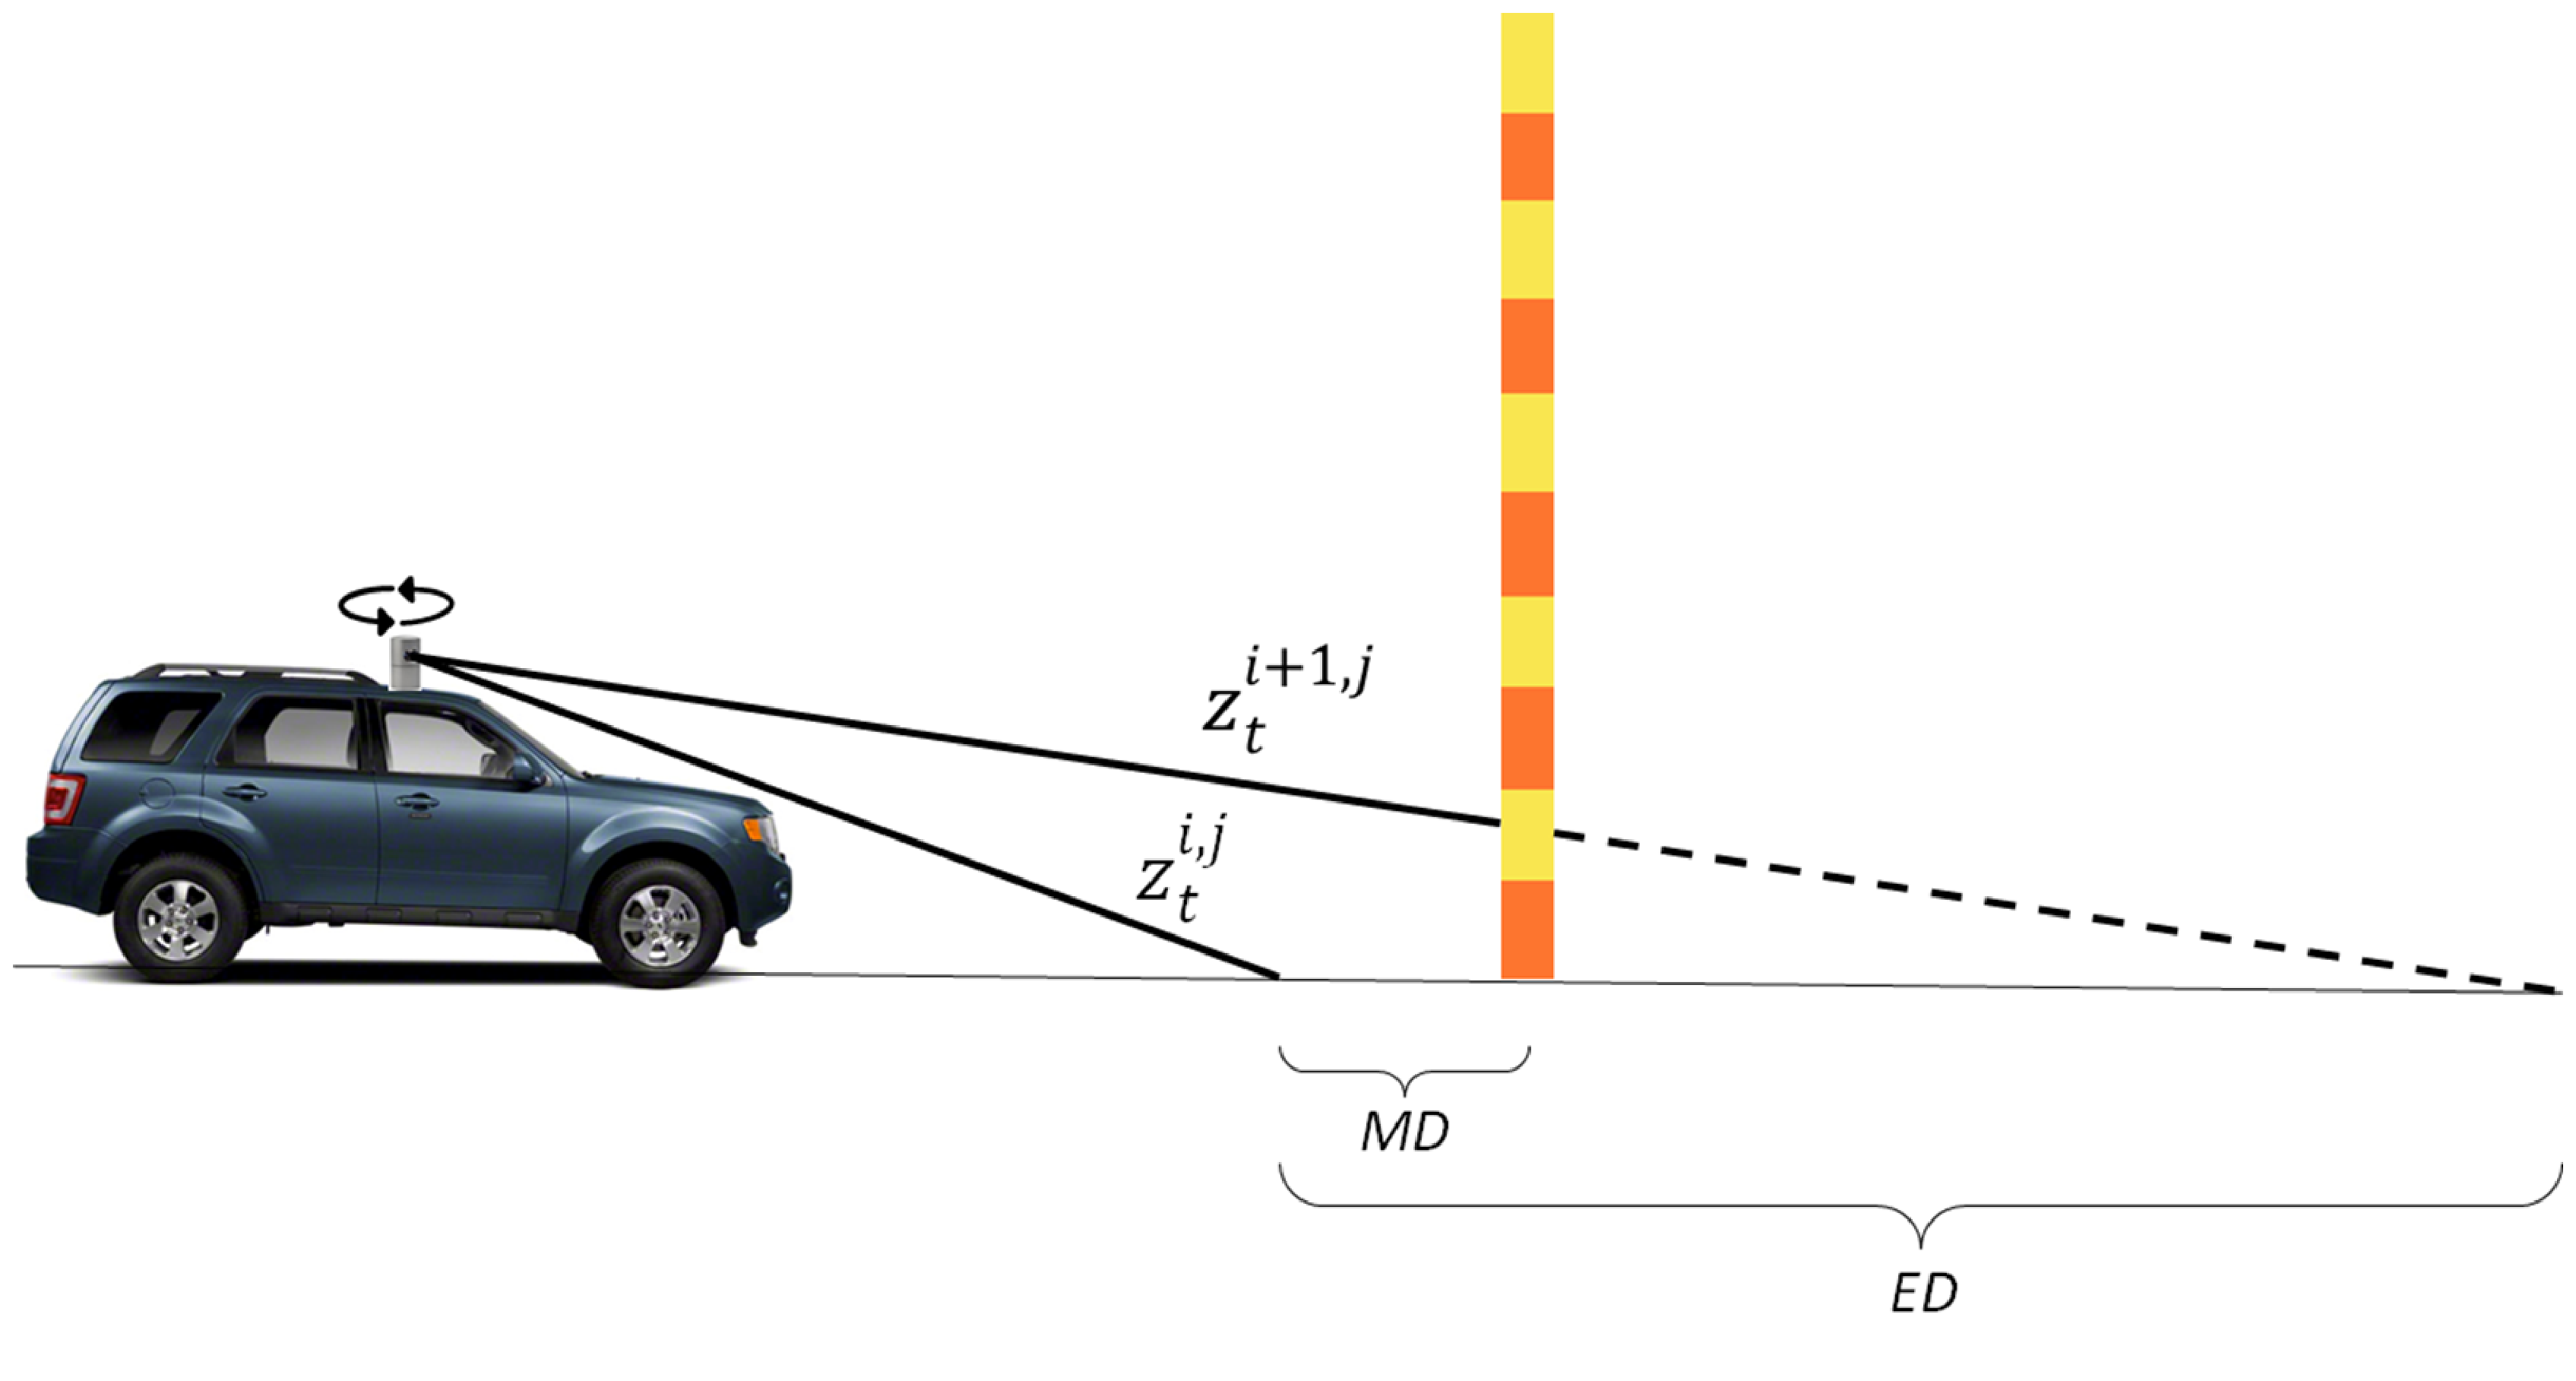
\includegraphics[width = 100 mm]{FIGURE06}
	\caption{Illustration of the obstacle detection scheme. Firstly, two consecutive Velodyne rays are projected on the ground. Then, the difference between the expected and the measured rays sizes on the ground are used to estimate the obstacle evidence.}
	\label{Fig::FIGURE06}
\end{figure}

The $MD(.)$ value is computed projecting two consecutive vertical rays on the ground and subtracting them:
\begin{equation}
\label{Eq::MeasuredDifference}
MD\left( z_t^{i,j},z_t^{i+1,j}\right) =\left| Pr\left( z_t^{i,j}\right) -Pr\left( z_t^{i+1,j}\right) \right|
\end{equation}
where  $Pr(.)$ is a ground projection function.

The expected difference value $ED(.)$ is calculated using a geometrical model of two vertical rays hitting the ground in an obstacle free environment. This geometrical model is illustrated in Figure \ref{Fig::FIGURE07}. In this Figure, $h$ represents the sensor height relative to the ground, $\alpha$ and $\beta$ are the vertical angles of ray $z_t^{i,j}$ and ray $z_t^{i+1,j}$, $b=Pr\left( z_t^{i,j}\right) $, $a=Pr\left( z_t^{i+1,j}\right) $, and $r$ is the length of the ray $Pr\left( z_t^{i+1,j}\right) $. The angles $\omega$ and $\gamma$ are auxiliary variables used in the $ED$ computation.

\begin{figure}[ht]
	\centering
	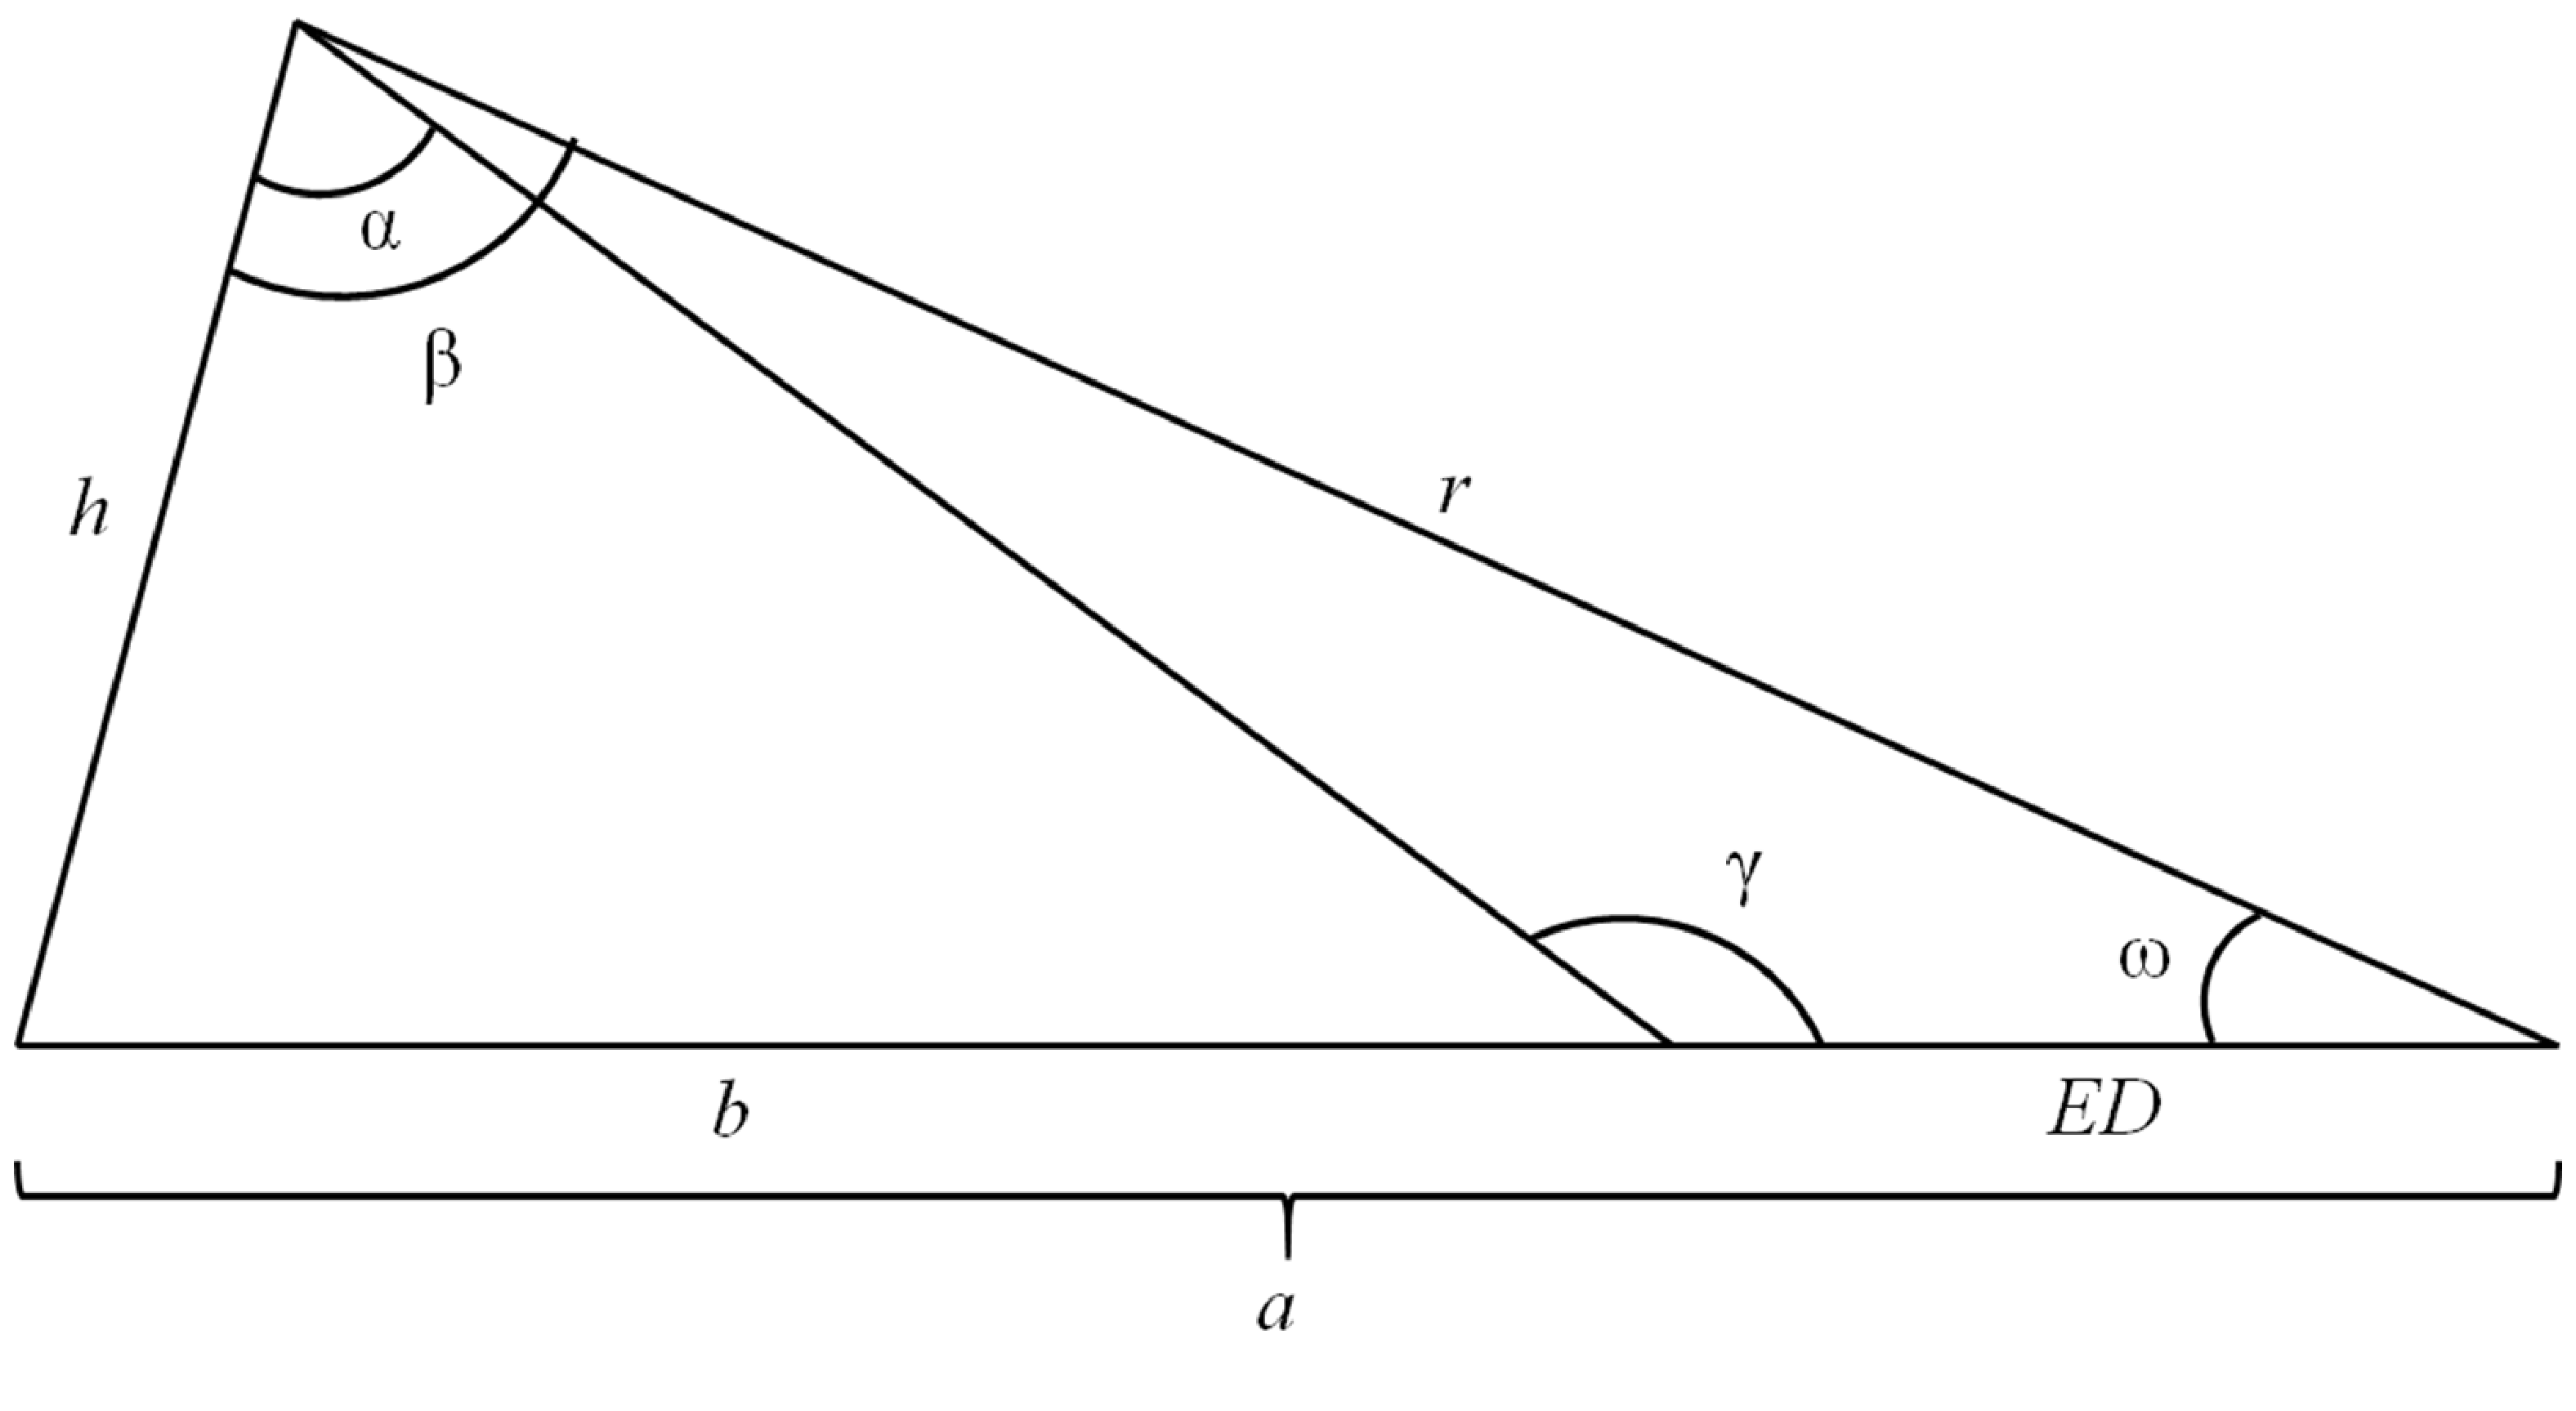
\includegraphics[width = 100 mm]{FIGURE07}
	\caption{Geometrical Model used to compute the expected value between two vertical 3D LiDAR rays projected on the ground.}
	\label{Fig::FIGURE07}
\end{figure}

The first step to compute $ED\left( z_t^{i,j},z_t^{i+1,j}\right) $ is to apply the sine law as follows:
\begin{equation}
\label{Eq::10}
\frac{\sin(\gamma)}{r}=\frac{\sin(\beta-\alpha)}{ED\left( z_t^{i,j},z_t^{i+1,j}\right)}
\end{equation}
and
\begin{equation}
\label{Eq::11}
ED\left( z_t^{i,j},z_t^{i+1,j}\right) = \frac{r\sin(\beta-\alpha)}{\sin(\gamma)}
\end{equation}
Then, the angle $\gamma$ can be computed by:
\begin{equation}
\label{Eq::12}
\gamma = \pi - \omega -(\beta-\alpha)
\end{equation}
The angle $\omega$ can be calculated by:
\begin{equation}
\label{Eq::13}
\frac{\sin(\beta)}{a}=\frac{\sin(\omega)}{h}
\end{equation}
and
\begin{equation}
\label{Eq::14}
\omega = \arcsin \left( \frac{h\sin(\beta)}{a} \right)
\end{equation}
After that, $a$ can be calculated using the cosine law:
\begin{equation}
\label{Eq::15}
a = \sqrt{h^2+r^2-2hr\cos(\beta)}
\end{equation}

Replacing the Equation \ref{Eq::15} in \ref{Eq::14}, \ref{Eq::14} in \ref{Eq::12} and \ref{Eq::12} in \ref{Eq::11}, the expected distance between two consecutive 3D LiDAR rays is given by:
\begin{equation}
\label{Eq::16}
ED\left( z_t^{i,j},z_t^{i+1,j}\right) = \frac{r\sin(\beta-\alpha)}{\sin \left( \pi -(\beta-\alpha) - \arcsin \left( \frac{h\sin(\beta)}{\sqrt{h^2+r^2-2hr\cos(\beta)}} \right) \right)}
\end{equation}

After computing the obstacles evidence $OE$, the occupancy probability $PO$ is given by:
\begin{equation}
\label{Eq::17}
PO = \frac{1}{\sqrt{2\pi\sigma_{OD}^2}}\exp \left( \frac{-OE\left( z_t^{i+1,j} \right)^2}{2\sigma_{OD}^2} \right)
\end{equation}
where $\sigma_{OD}$ is the obstacle detection standard deviation. The value was found during empirical experimental tests (in this work, we used $0.8$).


\subsection{Dead-Reckoning based on Scan-Matching}

The dead-reckoning is an important part of our system that detects intersection. It is used to place the Velodyne scan in the local map during the mapping. Mistakes to pose these scans can generate errors in the placement of the rays on the map. These problems in general happen because the car odometer may have bias, pour measurement and wheel slips. 
%If the car kinematic model is based on the steering model, to estimate the car steering-wheel bias can be a hard task, since inclinations on the ground would affect the calibration in different scenarios. This way, an alternative for having better pose estimation by the dead-reckoning is applying the gyros model instead
In normal condition (without rain), the slips does not affect so much the dead-reckoning in asphalt roads. But, in different sort of terrain such as grass, rocks, and soil, which has different friction coefficient, the slips are unpredictable and if they are wet it becomes worse. Alternatively, the ground type could be detected by processing the camera installed on-board, but the light condition limited its application. Note, this slips estimation is very important for vehicles that operate in mines, farms, desert or off-road since the ground is frictionless \cite{woodsterrain}.

Therefore, a scan matching has been applied between two Velodyne's point clouds in order to estimate the dead-reckoning. I.e., this system computes the car odometries (car speed and angular velocities) using only Velodyne imageries. It is well known as Visual-LiDAR Odometry \cite{Zhang_LOAM, Zhang_V-LOAM, zhang2014real}. It begins with the car stationary registering the scans, whenever the car starts to move the difference between the pose will be used to calculate the odometries, with them predictions of the car movement will be computed to generate initial guesses for later scan-matches.

Another fact, The Velodyne HDL32-E spins 20 times per second scanning with 32 laser shots that take 46.09 $\mu$sec, so, for each $360^{o}$ scan, the Velodyne takes 50 msec. If the car speed is about 10 m/s, the car will travel around 0.5 meter to complete one full $360^{o}$ scan. This way, if the car speed and turn are not considered to pose every 32 laser shots in the right place, the same static objects in consecutive revolution is going to be in different places in the world. Consequently, the quality of the matching will degrade.

In this works, the Generalized-ICP (GICP) has been applied to provided the matches. We considered the GICP to perform point cloud registration since it was designed to work with Velodyne points \cite{58segal2009generalized}. Usually, the GICP has problems to work on-line using dense point clouds as the Velodyne one. Thus, using a the whole points of the spins, the time to process one frame is over 0.5 seconds. To reduce the computational time, a 3D voxel-grid operation has been employed with a grid-size of 0.6 meters. Now, it may register 10 frames per second.  Figure \ref {Fig::Dead_reckoning} shows Visual-Lidar Odometry path (dead-reckoning) (green) compared against to the GPS (red).

\begin{figure}[ht]
	\centering
	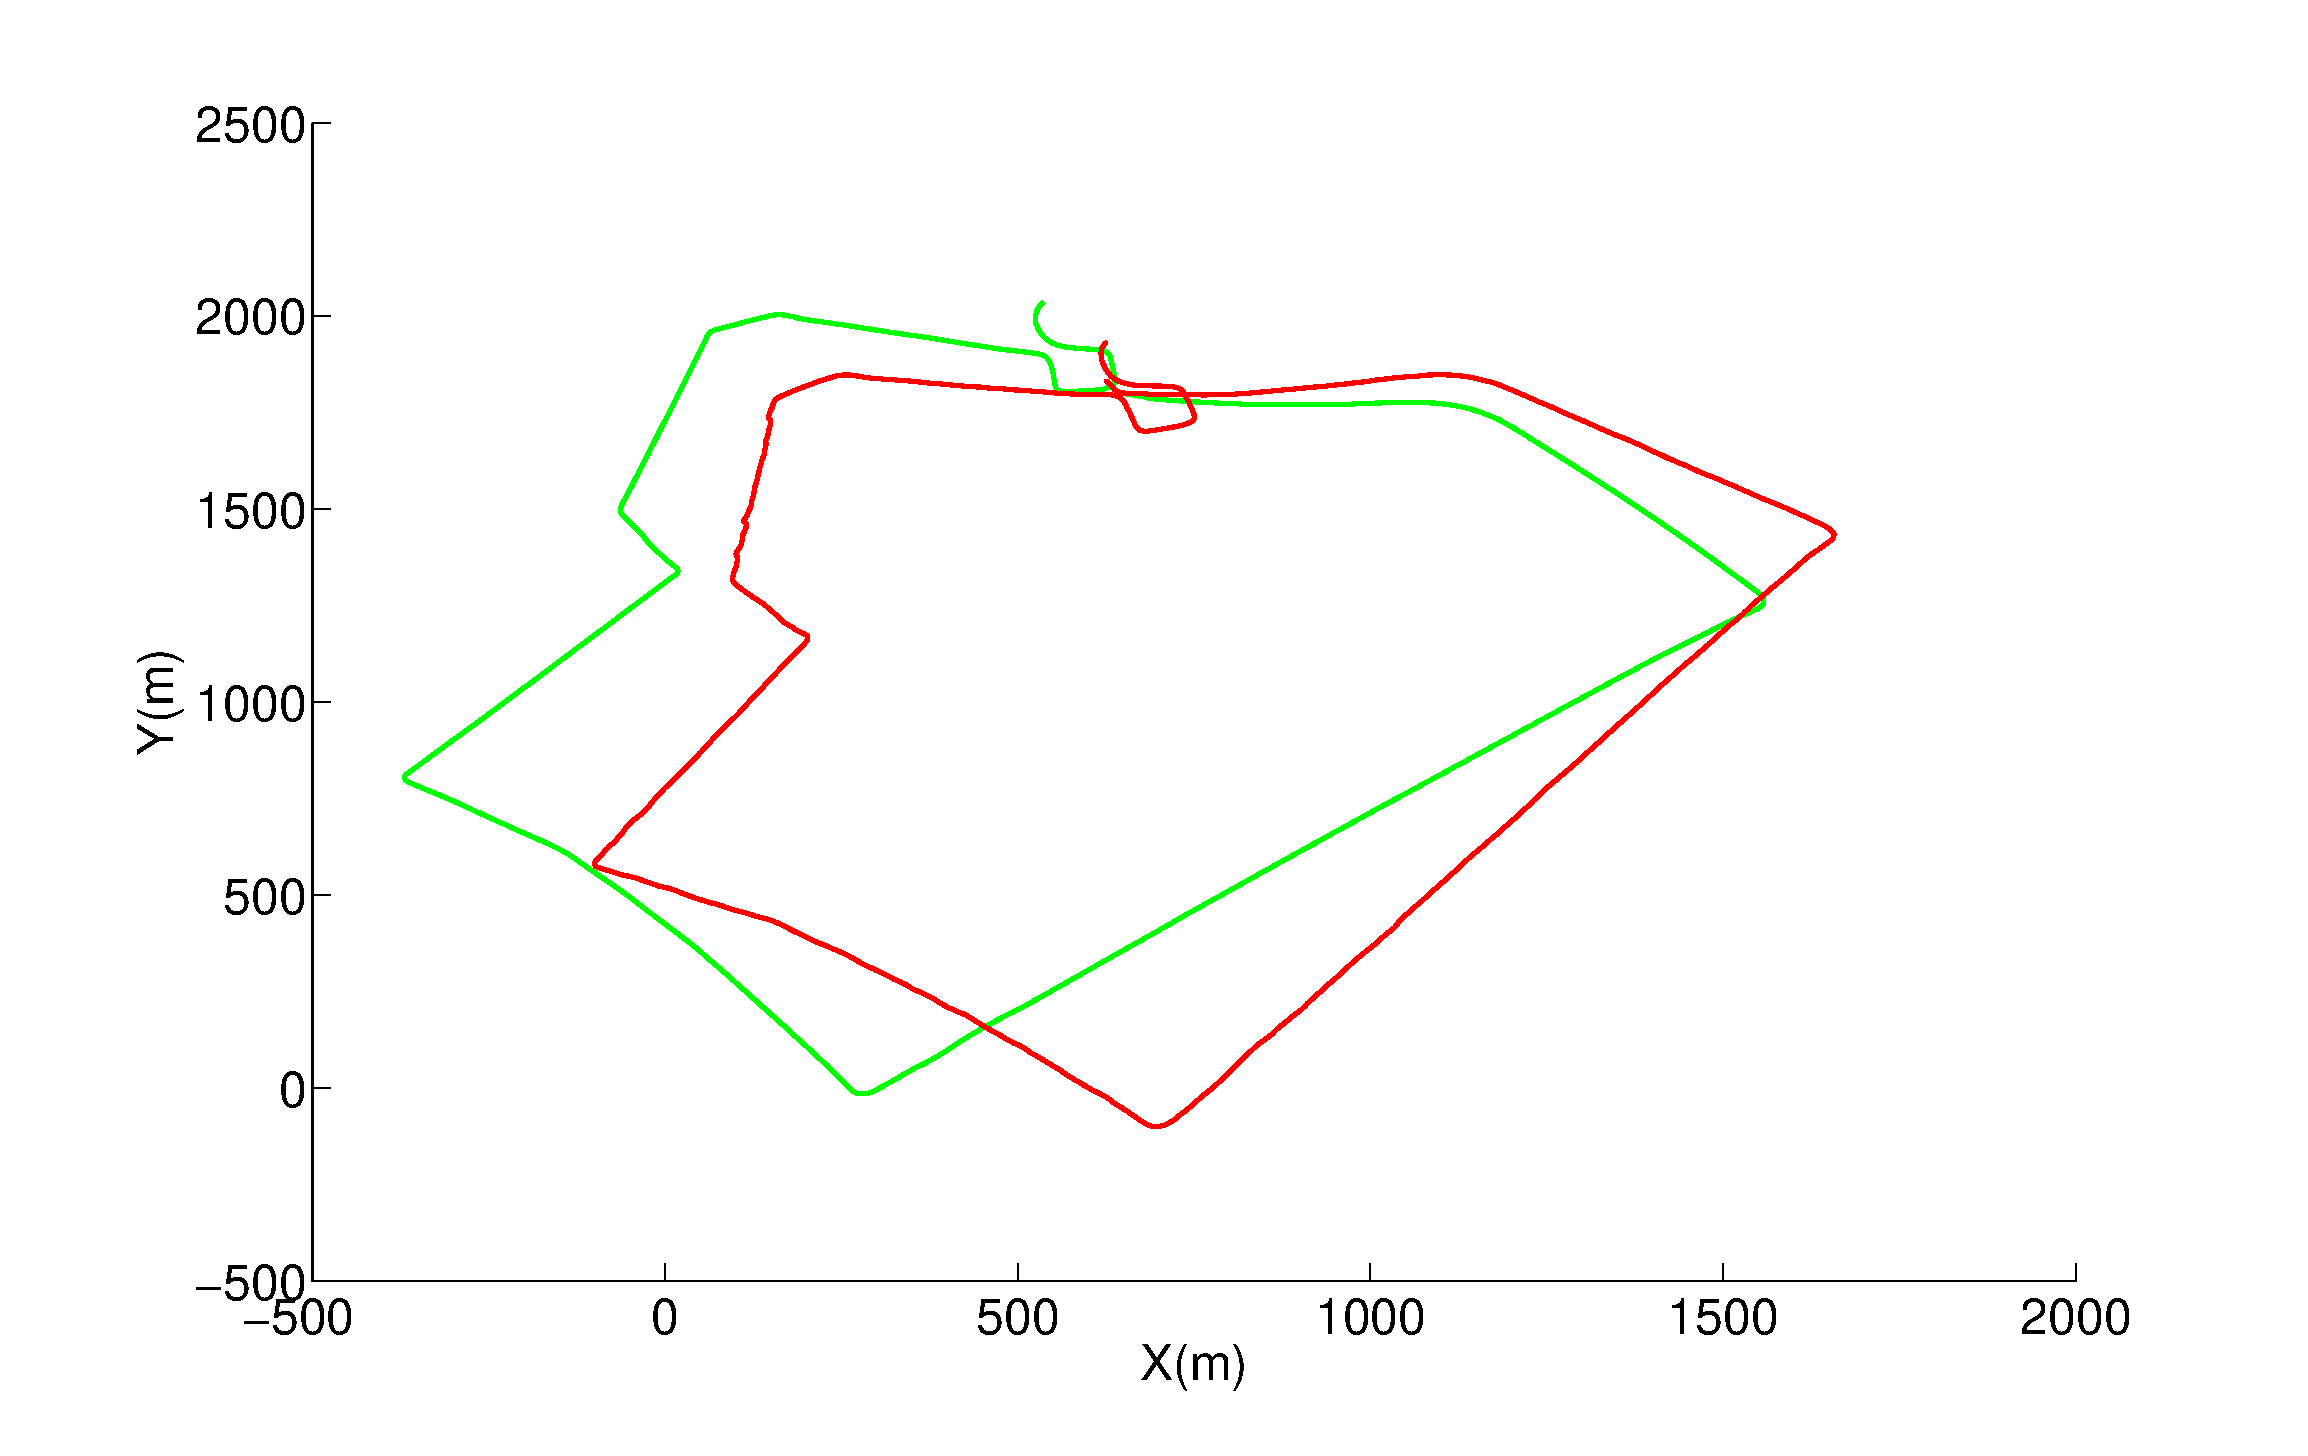
\includegraphics[width = 150 mm]{Dead_reckoning.eps}
	\caption{The car dead-reckoning estimated by the Visual-Lidar Odometry. The green and red lines represent the dead-reckoning and GPS respectively.}
	\label{Fig::Dead_reckoning}
\end{figure}



\subsection{Normalized Mutual Information}

The Normalized Mutual Information (NMI) is a variant of Mutual Information that has the capacity for measuring different types of relationships between variables [14]. NMI has been used to measure the relation between images captured from different sources. For instance, this probabilistic distance is widely used in medical image registration, where the pictures are taken from different devices with dissimilar color spectrum [18]–[20]. 

Because the aerial image map and the re-emission map also originate from devices with different image construction principles, in this work, the NMI metric is used to measure the distance between an aerial image map ($m$) and a re-emission local map ($m_{local}$). The NMI distance is defined as follow:
\begin{equation}
\label{Eq::NMI}
NMI(m_{local},m)= \frac{H(m)+H(m_{local})}{H(J(m_{local},m))}
\end{equation}
where $H(m_{local})$ is the entropy (Eq. \ref{Eq::HIST1}) of $m_local$, $H(m)$ is the entropy of $m$ and $H(J(m_{local},m))$ is the joint entropy (Eq. \ref{Eq::JHIST}) of both maps. The NMI value of maximum dissimilarity is close to 0 and the maximum similarity is around 2. Entropy values are calculated considering histograms with 255 bins, as follows:
\begin{equation}
\label{Eq::HIST1}
H(A)= -\sum\limits_{i=0}^{255}p_A(a_i)\log p_A(a_i)
\end{equation}
\begin{equation}
\label{Eq::PROB1}
p_A(a_i)= -\frac{a_i}{\sum\limits_{i=0}^{255}a_i}
\end{equation}
\begin{equation}
\label{Eq::JHIST}
H(J(A,B))= -\sum\limits_{i=0}^{255}\sum\limits_{j=0}^{255}p_{J(A,B)}(jab_{ij})\log p_{J(A,B)}(jab_{ij})
\end{equation}
\begin{equation}
\label{Eq::PROB2}
p_{J(A,B)}(jab_{ij})= -\frac{jab_{ij}}{\sum\limits_{i=0}^{255}\sum\limits_{j=0}^{255}jab_{ij}}
\end{equation}

Here, $A$ represents the histogram of $m_{local}$ or $m$. $p_A(a_i)$ is the probability of the pixel intensity $i$ appear into the map image, i.e. the value $a_i$ of the histogram normalized by the sum of the histogram values. $J(A,B)$ is a joint histogram, which denotes the combination of intensity values for corresponding pixels of the two images $m_{local}$ and $m$ [21]. $p_{J(A,B)}(jab_{ij})$ is the probability of the combination of the pixel intensities $i$ and $j$ appearing in the joint histogram, i.e. the value $jab_{ij}$ under the intensity combination $i$ and $j$ of the joint histogram $J(A,B)$ normalized by the sum of the histogram.

\subsection{Particle Filter Localization Approach Improved By Normalized Mutual Information}

In order to localize the vehicle accurately using maps, we apply a Particle Filter Localization (PFL) strategy [16]. During initialization, it spreads particles in the workspace, i.e. over the whole map or using an initial guess like the GPS information or manual annotation. Thereafter, it recursively predicts the robot movement and corrects the prediction using the captured environment data.

The sample motion model is responsible for estimating hypothetical movements (i.e., predictions) of the particle $k$ from $x_{t-1}^k$ to $x_t^k$. This phase involves sampling from the state transition distribution $p(x_t^k |u_t,x_{t-1}^k,m)$ considering the vehicle state $u_t=\left\langle v_t,\omega_t\right\rangle$ (vehicle speed and angular velocity at time $t$, respectively) received from the car odometry. The sampling process is performed based on predictions following the Ackerman kinematic model having $v_t$ and $\omega_t$ disturbed by a Gaussian noise [22]:

\begin{equation}
	\label{Eq::Ackeman}
	\left( \begin{array}{c} x\\ y\\ \theta \end{array} \right)_t = 
	\left( \begin{array}{c} x\\ y\\ \theta \end{array} \right)_{t-1} +
	\left( \begin{array}{c} 
	v_t \Delta t \cos(\theta_{t-1})\\ 
	v_t \Delta t \sin(\theta_{t-1})\\ 
	\omega_t \Delta t \end{array} \right)
\end{equation}

After the initial process of spreading particles, the particle's weight, $w_t^k$, is computed applying Eq. \ref{Eq::NMI} between the $m_{{local}_t}$ and $m$ given $x_t^k$. To this end, $m_{{local}_t}$ is placed in m coordinates using the current position of the robot (given by the dead-reckoning) and $x_t^k$. The computation of Eq. \ref{Eq::NMI} is performed between every particle to measure the distance between the a priori map m and the local map $m_{{local}_t}$. The final value of $w_t^k$ is normalized by the maximum and minimum values from Eq. \ref{Eq::NMI}. Finally, the best particles are re-sampled based on their weights. For calculating the final pose, the average of the best selected particles' pose is used.


\section{Road-Map Localization System Architecture}

Road-Map Localization System (RMLS) is Monte Carlo Localization (MCL) that fuses the dead-reckoning with road map information to produce a car global position. The MCL is probabilistic localization approach, which follows the recursive nonparametric Bayesian Filter, also known as Particle Filter Localization. Furthermore, RMLS implements intersection observability to enhance the vehicle global position in GPS-denied scenarios. This system works only with the 3D LiDAR (Velodyne HDL-32E) information, since we are proposing odometer system based just in LiDAR information called Visual-LiDAR Odometer to estimate the car dead-reckoning. 

Figure \ref{Fig::RoadMap-system} illustrates Road-Map Localization System architecture. Initially, the system initializes the MCL particles as Gaussian distribution centered in the first car position. The primer pose is indicated manually by the system operator. This is the only external information received. Then, for each car pose given by odometries, the RMLS attaches it in buffer (car path) with last 200 observability (i.e. only when the car is moving). Hence, the particles compute their weight comparing the car path against the road map. 

The odometries are computed by our Visual-LiDAR Odometer sub-system based on Generalized Iterative Closest Point (GICP) \cite{58segal2009generalized}. It does so, registering two consecutive Velodyne scans to indicate the car movement, and the difference between the old pose and current one is taken to produce the odometries. Then, the sub-system publishes the odometries to the other, beyond to uses itself to predict the vehicle movement to the next frame. 

 
\begin{figure}[t!]
    \centering
    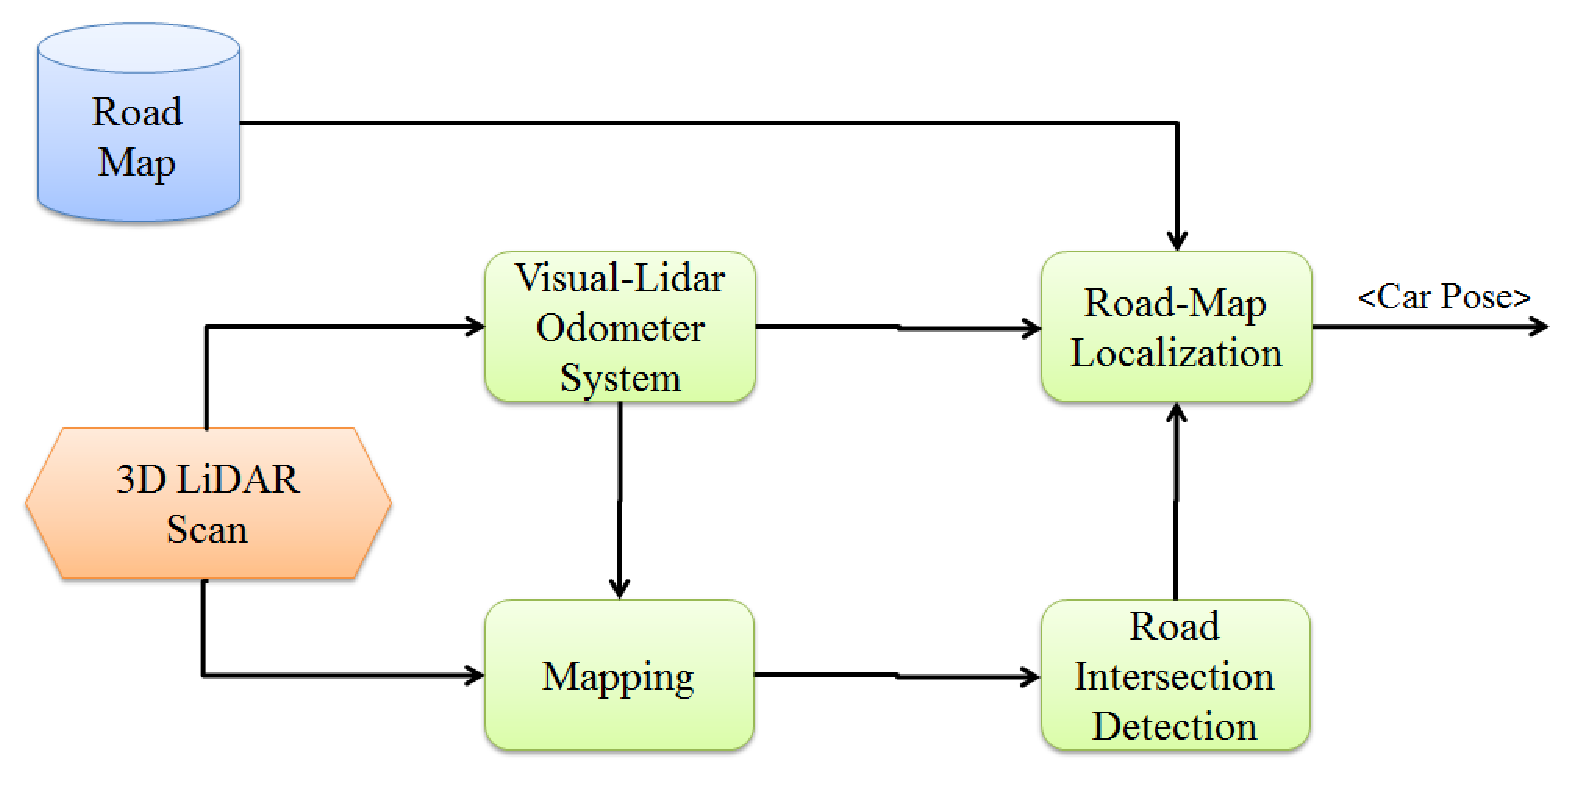
\includegraphics[width = 150mm]{RoadMap-system2.eps}
    \caption{Road-Map Localization System architecture. The system consists in road map and LiDAR sensing every instant that is used to estimate the car Odometries by Visual-LiDAR Odometer. Then, it uses this information to build re-emission and occupancy grid map locally as well as to build car path to compare against the road map. The maps are used by Road Intersection Detection sub-system to measure the road width, and inform whether car is crossing a road junction. The intersection observability is fused with distance between the dead-recking and road map by Monte Carlo Localization. Finally, the MCL computes the car pose selecting and summarizing the particles.}
    \label{Fig::RoadMap-system}
\end{figure}

To detect a road intersection formerly the 3D LiDAR data should be processed to produce local grid maps. The mapping builds a occupancy and re-emission grid map posing the lasers using dead-reckoning given by Visual-LiDAR Odometer. The Re-emission grid map is produced using the infrared LiDAR reflectance taking the average of re-emission value of each ray lied in a grid-cell. On the other hand, The occupancy map is made classifying whether a laser beam touch a obstacle or not. The both maps are used by the Road Intersection Detection sub-system to measure the road width and inform to MCL if the car is crossing a road junction. With this information, the MCL attributes a likelihood for each particle that is placed in intersection on the road-map. In the end, the particles are re-sampled by weight computed through intersection observability and comparison between the car path and road map. The selected ones are used to compose the car pose in the instant $t$.    


%Each particle poses the car path according to its position, and then it computes the weight. The road map could be downloaded from the Internet (Google or Bing maps), or produced by a segmentation on the area photographs.

\section{Bayesian Localization}

Bayesian methods \cite{Arulampalam02atutorial} allow adequate processing for dynamic state estimation problems. Bayesian approaches aim at synthesizing the probability density function (PDF) of the state vector based on all the available information. Consequently, vehicle global  localization can be treated as a Bayesian estimation problem, where the estimated variable is the pose of the vehicle. If the vehicle's pose (in the case of 2D localization) at time $k$ is expressed through the 3 DoF vector 

\begin{equation}
\label{Eq::ch2-1}
X_k = [x_k, y_k, \theta_k]
\end{equation}

then the localization problem implies the recursive synthesis of the PDF

\begin{equation}
\label{Eq::ch2-2}
p_{X_k, | z^{\left( k\right)}} = \left( X_k, | z^{\left( k\right)}\right) 
\end{equation}

where $z^{\left( k\right)}$ represents the sequence of all the available observations until time $k$.

If the posterior $p\left( X_{k-1} | z^{\left( k-1\right)}\right)$ $\left( *\right)$ at time $k-1$ is available, then the prior at time $k$ (due to a prediction step) is:

\begin{equation}
\label{Eq::ch2-3}
p\left( X_{k} | z^{\left( k-1\right)}\right) = \int  p\left( X_{k}, X_{k-1}\right) \cdotp p\left( X_{k} | z^{\left( k-1\right)}\right) \cdotp dX_{k-1}   
\end{equation}

where the conditional PDF $p\left( X_{k}, X_{k-1}\right)$ is provided by the process model of the system (in this case the kinematic model of the vehicle).

At time $k$ a set of measurements,  $z^{\left( k\right)}$, become available, consequently allowing the synthesis of a posterior that is obtained through a Bayesian update stage,

\begin{equation}
\label{Eq::ch2-4}
p\left( X_{k} | z^{\left( k\right)}\right) \propto p\left( X_{k} | z^{\left( k-1\right)}\right) \cdotp p\left( z^{\left( k\right)} | X_{k}\right)
\end{equation}

where $p\left( z^{\left( k\right)} | X_{k}\right)$ is the likelihood function associated to observation $z=z^{\left( k\right)}$.

For nonlinear non-Gaussian estimation problems, there are usually no analytic expressions for the estimated PDFs. A common approach for treating these problems is the Particle Filter (PF), that is able to estimate non-Gaussian and potentially multimodal PDFs. The generated PDF is represented through a set of samples (particles) with associated weights, and the estimates are computed based on these samples and weights. Details about PF can be found in \cite{Thrun:2005:PR:1121596, Thrun00j}

\section{Constrained Localization in Segment-Based Maps}

The system for localizing the platform is based on a process model and a set of likelihood functions that allow implementing the prediction and update steps of a PF. The process model is the kinematic model of the autonomous car employed in the experiments. And, in the context of this paper, there are two definitions of likelihood functions that are associated with the road segments: the Base Likelihood and the Extended Likelihood. The Base Likelihood is intended to model the likelihood of a position, i.e. the likelihood of a point being located on a valid road, while the Extended Likelihood (or path likelihood) is the likelihood of a path coinciding with a valid road. Both definitions of likelihood function are based on the segments defined in the road map.

\subsection{Base Likelihood Associated with the Road Map}

For a set of particles at time $k$, $\left\lbrace X_{k}^{i},w_{k}^{i} \right\rbrace _{i=1}^N$, the Base Likelihood (BL), $L_B\left(X_{k}^{i} \right)$, associated with a given map (set of segments) is defined as follows:
\begin{equation}
\label{Eq::ch2-5}
L_B\left(X\right) =p\left( map | X\right) = \max_{j=1}^{N}\left\lbrace f\left( X,S_j,C_j \right) \right\rbrace 
\end{equation}
where $\left\lbrace  S_j \right\rbrace_{j=1}^N$ represents the set of segments that compose the road map and $C_j$ denotes the properties of segment $S_j$ (road's width, number of lanes, lane directions, etc.). The function $f(\ldotp)$ is highly dependent on the distance between the pose component (of the state $X$) and the segment $S_j$. The function $f(\ldotp)$ may be also dependent on certain segment's properties such as its width and circulation direction.

A simplified version of \ref{Eq::ch2-5} is
\begin{equation}
	\label{Eq::ch2-6}
	L_B\left(X\right) =	p\left( map | X\right) = \left \{
		\begin{array}{l}
			1;\ if\ X\ \in\ \Omega(map,\Omega_k)\\\\
			0;\ if\ X\ \ni\ \Omega(map,\Omega_k)
\end{array}
\right.
\end{equation}
where the region $\Omega_k$ is a convex hull (usually just a rectangle) that contains the current set of particles at time $k$, i.e. $\left\lbrace  X_k^i \right\rbrace_{j=1}^N$.

The region $\Omega(map,\Omega_k)$ defines the roads as thick bands using the segment's locations and their associated properties provided in the road map definition. $L_B(X)$  is defined just on a small convex region of interest (ROI), $\Omega_k$, which is big enough to contain all the current particles. Through the dynamic definition of a moving and resizable ROI, the likelihood function $L_B(X)$ can be evaluated for all of the particles in real time at low computational cost.

\subsection{Extended Likelihood}

For improving the performance of the estimation process in the presence of out-of-map situations, an extended likelihood function is defined. An out-of-map situation occurs when the vehicle is traveling through unknown sections of the map, i.e. sections of the environment that are not included in the road map. 

Particles will tend to cluster towards regions of high Base Likelihood, which are assumed to be consistent with the map (e.g. existing roads in the map). This can be an adequate behavior in cases where the map is complete and the vehicle remains on it permanently. However, in certain cases, the vehicle might travel through roads that are not present in the road map. For those cases, the convergence of the localization process can be improved by using the recent history to build an estimated dead-reckoning path.

An estimated dead-reckoning path for each particle at time $k$ can be efficiently computed by combining dead-reckoning (obtained from an independent estimation process) with the current value of the particle $X_k^i$. This estimated path is only realistic for short time horizons, as dead-reckoning is accurate only for short time horizons. So, given a particle $X_k^i=[x_k^i,y_k^i,\theta_k^i]$ and recent dead-reckoning information, an estimated dead-reckoning path (it is actually a trajectory as well, since there is also time information), $\xi_i (t'), t' \in [k-\tau,k] $ is synthesized, where the value $\tau$ defines some short horizon of time. This path ends exactly at the current pose (i.e. matching position and heading) of the particle, i.e. $\xi_i(k)=X_k^i$.

The estimated dead-reckoning path is usually defined in a different coordinate system, as it is the result of an independent process (it could even be expressed in a completely uncorrelated coordinate frame). One important aspect of the estimated dead-reckoning path is its quality given a specific coordinate system, i.e. if its shape is, after proper rotation and translation, similar to the real path of the vehicle. If the estimated dead-reckoning path is expressed as the path $\mu^i (t' )=(x_{\mu}(t'),y_{\mu}(t'),\theta_{\mu}(t'))$, then the process of associating it with an individual particle and of mapping it into the global coordinate frame is performed simply by applying the rotation and translation defined by the current particle position and heading (see details in \cite{guivant2010robust}).

The Extended Likelihood (EL) of a particle is given by the line integral of the BL function along the estimated dead-reckoning path:
\begin{equation}
\label{Eq::ch2-7}
L_E (X_k^i )=\int_{k-\tau}^{k} L_B(\xi_i(t')) \cdotp dt',
\end{equation}
where $L_B (\xi)$ is the BL function of the point $\xi$, (as it was defined in \ref{Eq::ch2-6}).

In order to avoid the influence of the vehicle speed on the path likelihood, we evaluate BL according to the arc length parameter $s$, integrating over the path, (i.e., in space and not in time):
\begin{equation}
\label{Eq::ch2-8}
L_E (X_k^i )=\int_{0}^{l_s} L_B(\xi[s]) \cdotp ds,
\end{equation}
where $\xi[s]$ is the path expressed as a function of its intrinsic parameter $s$, and $l_s$ is the length of path. The continuous line integral of the path can be approximated by its discrete version,
\begin{equation}
\label{Eq::ch2-9}
L_E (X_k^i )=\sum_{j=1}^{N_J} L_B(\xi[s_j]) \cdotp ds,
\end{equation}
where the samples of the intrinsic parameter, $s_j$, are densely distributed over the estimated dead-reckoning path.

Some additional refinements can be considered for the definition of BL \ref{Eq::ch2-5}. For instance, one can consider the direction of the road. In this case, BL would not be just a function of the position, but it would depend on the vehicle heading at each point of the path. A path's segment that crosses a road would add to the likelihood if it crosses the road in the proper direction.

Figure \ref{Fig::ROI} shows a synthetic example of BL (shown in gray), particles that represent the pose of the vehicle, and their associated estimated dead-reckoning paths (in cyan). The particles' positions and headings are represented by blue arrows. The red path corresponds to the most likely hypothesis (according to the Extended Likelihood measure).

\begin{figure}[th]
\centering
    \subfloat[]{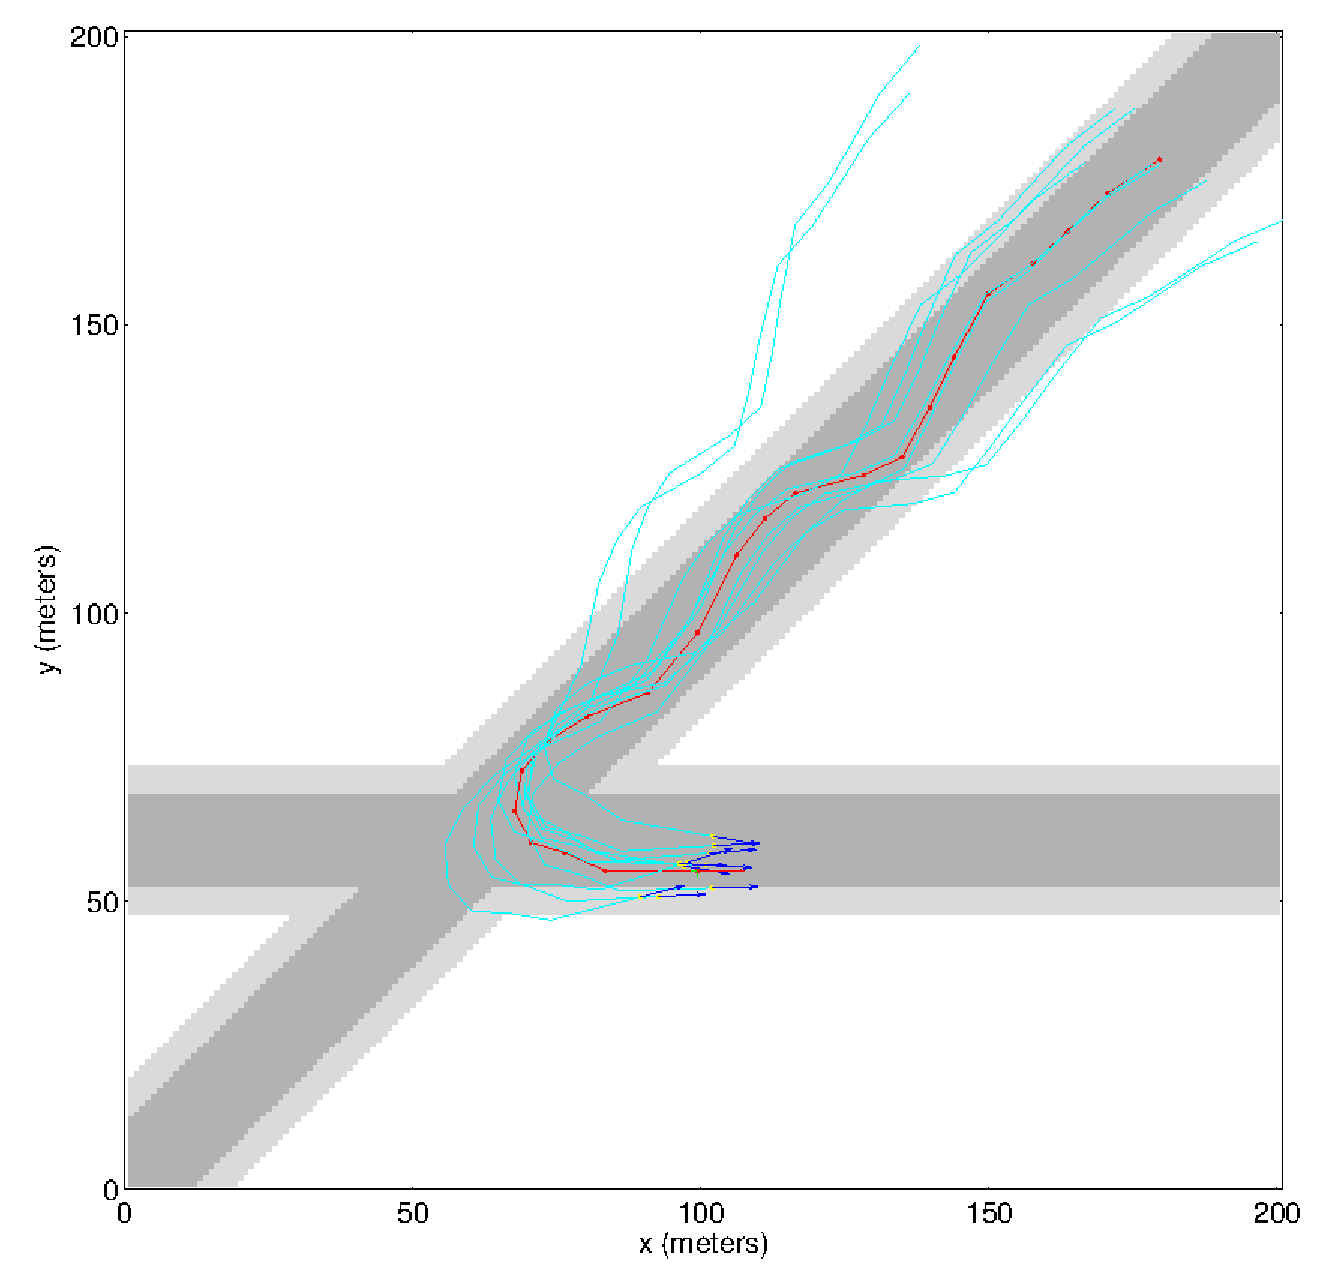
\includegraphics[width=50mm]{VGPSFig11.eps}
    \label{Fig::ROI1}}
    \subfloat[]{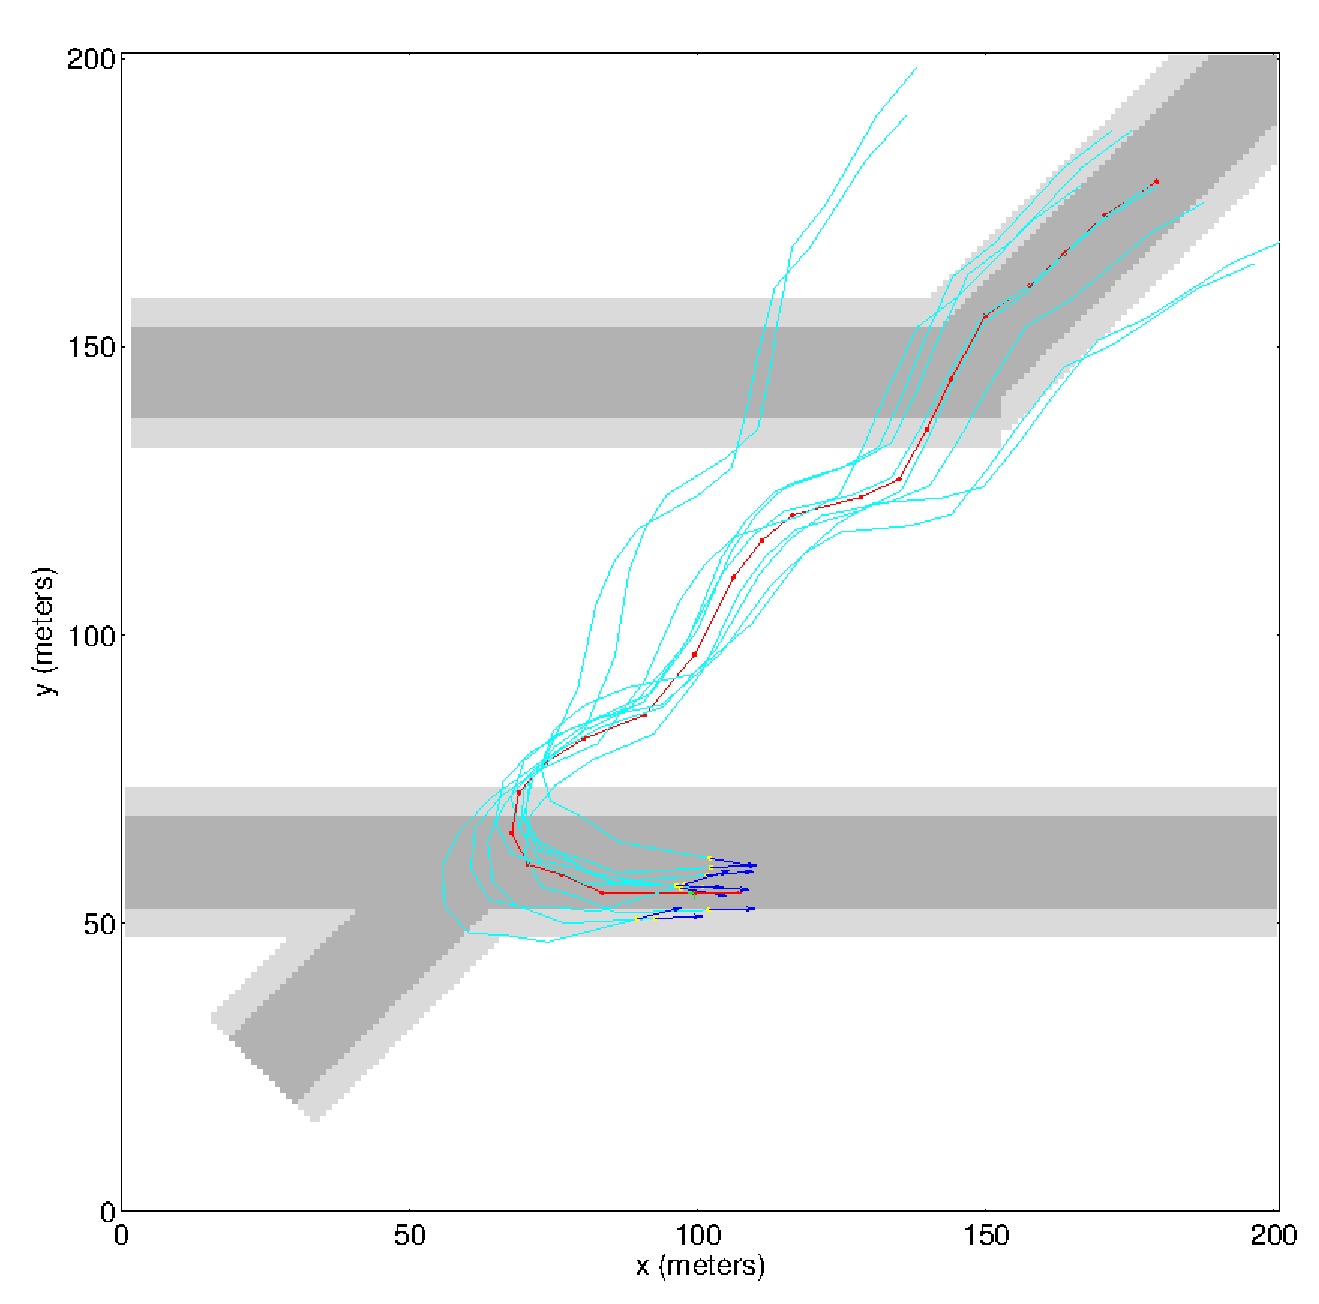
\includegraphics[width=50mm]{VGPSFig22.eps}
    \label{Fig::ROI2}}\\
    \subfloat[]{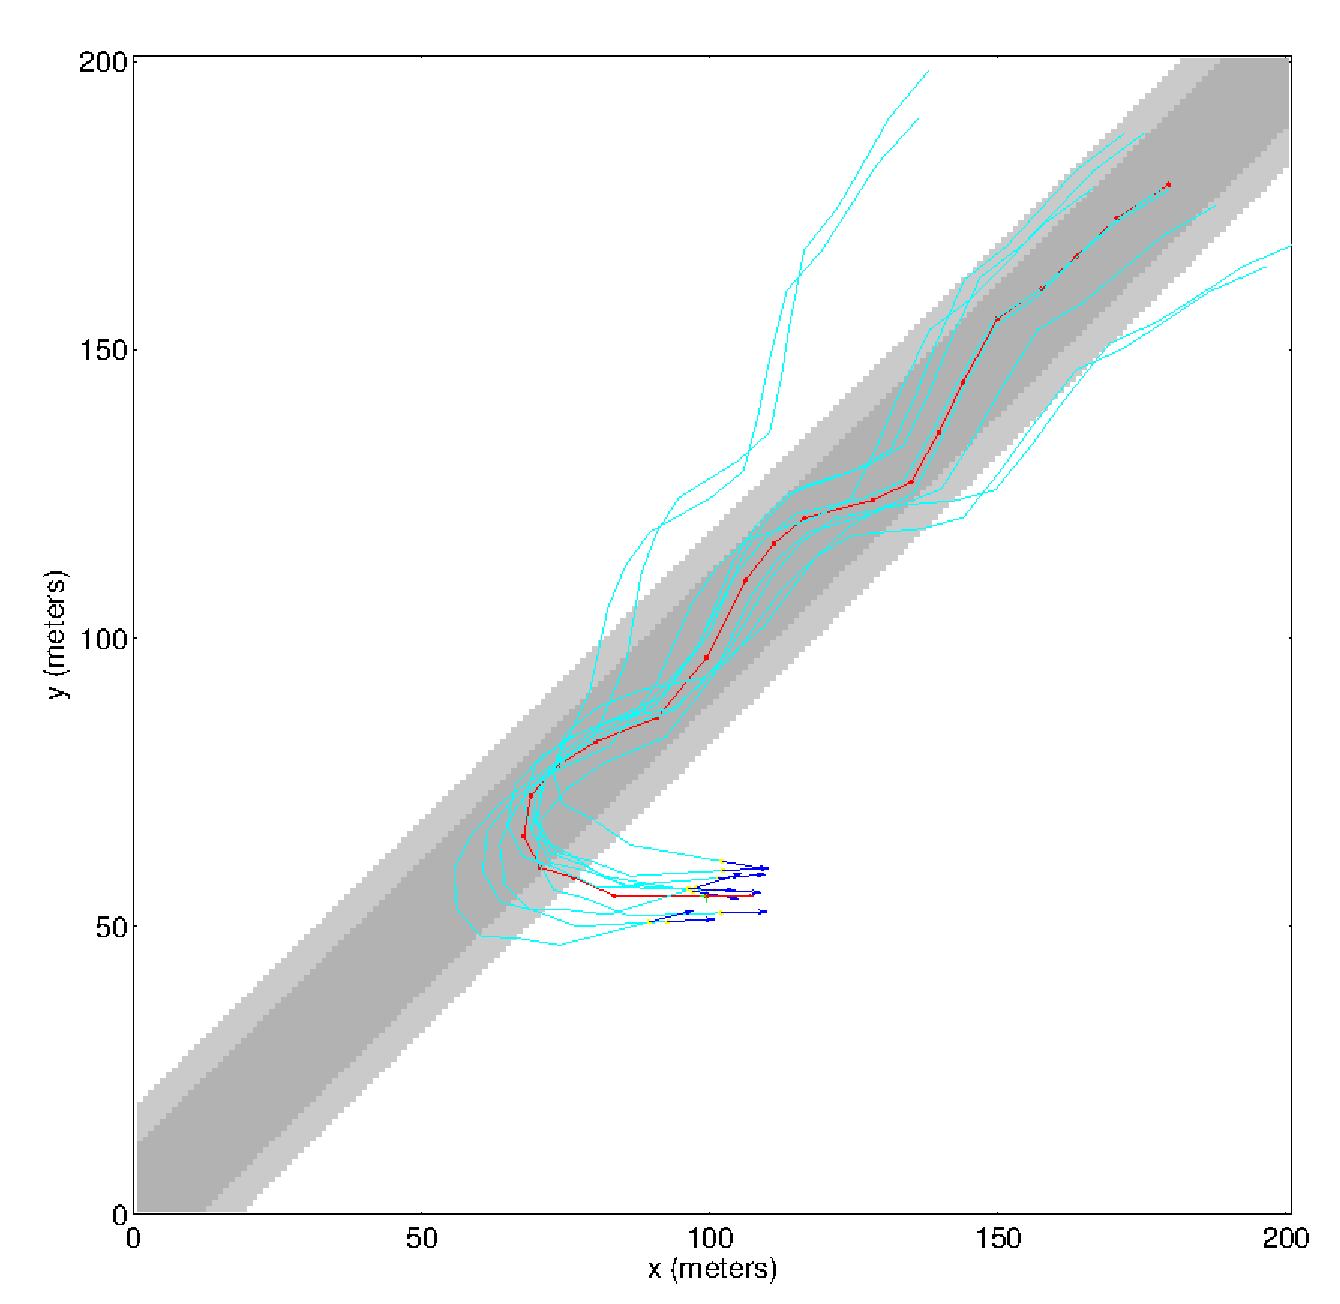
\includegraphics[width=50mm]{VGPSFig33.eps}
    \label{Fig::ROI3}}
    \subfloat[]{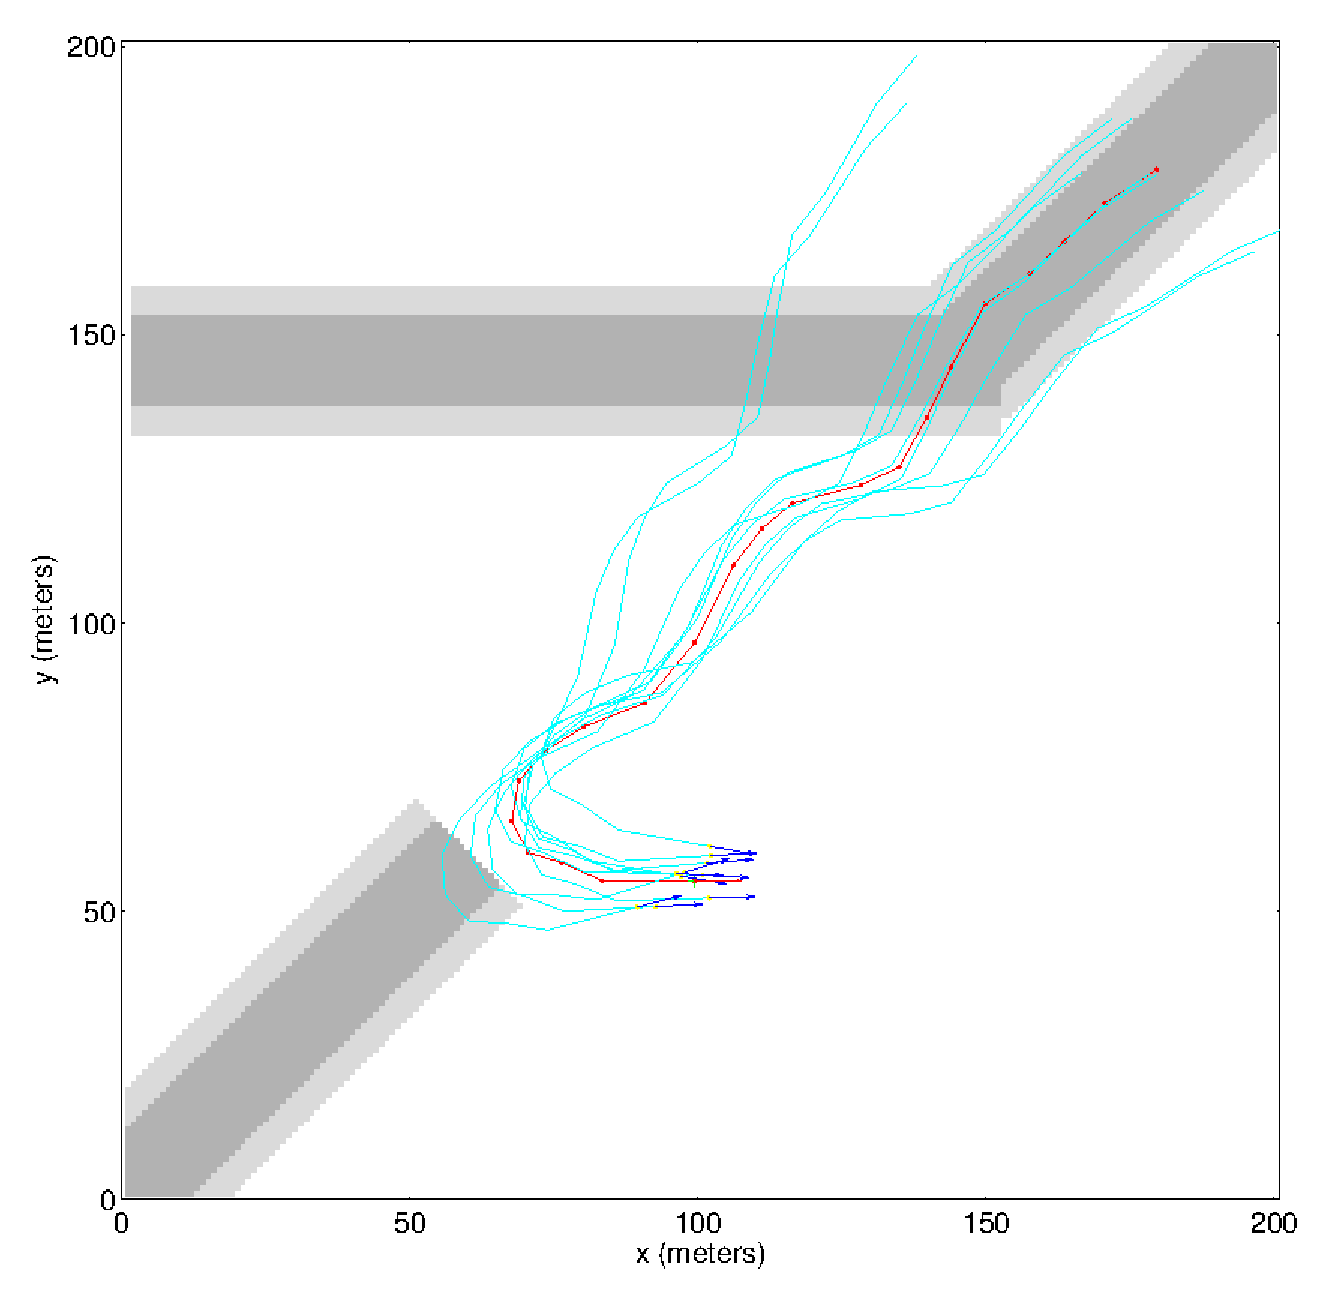
\includegraphics[width=50mm]{VGPSFig41.eps}
    \label{Fig::ROI4}}
\caption{Synthetic examples for a ROI of $200m\times200m$. The value of the Base Likelihood ($L_B(X)$) is shown in gray (the darker, the higher). A set of particles and their associated paths are included. The particle and path with maximum extended likelihood, $L_E(X_k^i)$ are shown in red. In three of the four cases, the vehicle temporarily abandons the road. In cases (b) and (c), all particles have equally low Base Likelihood; however, many particles still have high Extended Likelihood. Images taken from \cite{guivant2010robust}.}
\label{Fig::ROI} 
\end{figure}

By using observations that consider the estimated dead-reckoning path, the out-of-map problem is mitigated. The transition between a situation where the vehicle is on the road map to another where it is completely out of it (i.e. current pose and estimated dead-reckoning path are outside the road map) can be performed safely by using an approach based on hysteresis, as discussed in \cite{guivant2007global,guivant2010robust}.

In the synthetic example shown in Figure \ref{Fig::ROI}, the region of interest (ROI) is a square of 200 by 200 meters. This ROI is big enough to contain the current population of particles and their associated estimated dead-reckoning paths. The most likely particles are those that have a path mostly inside the road. In the case of Figure \ref{Fig::ROI4}, although all particles are located on the road (high Base Likelihood), many of their associated paths have large segments outside the zones of high Base Likelihood. In Figure \ref{Fig::ROI2} one can see the remarkable effect that a wrong heading direction may cause. This situation is also illustrated in \ref{Fig::ROI3}.

When the filter infers that the vehicle has been outside the map for sufficient time (i.e. no particle shows relevant part of their estimated dead-reckoning paths inside the road map), no updates are performed on the particles, i.e. the filter works in pure prediction mode. When the vehicle enters the road map again and there are enough particles with the required EL, i.e. higher than certain threshold, then the filter restart to apply updates on the particles. However, this transition typically is not immediate. There could be some delay until the required estimated dead-reckoning paths are consistent with the road map -- the fact that a particle is well inside a road of the road map does not mean that its likelihood should be high. It needs a relevant fraction of its associated estimated dead-reckoning path inside roads of the road map in order to be considered ``inside the road map''.


\subsection{Likelihood Based on Real Sensing Capabilities}

The previously defined likelihood functions are not based on real measurements (provided by sensors), i.e. the likelihood functions $L_B(x)$  and $L_E(x)$ are just based on the hypothesis that the vehicle is usually traveling on the roads of a known road map.

If the vehicle is equipped with proper sensors, it might be able to infer when it is effectively on a road or not (even though the road may not be part of the road map). This inference process could be based on 3D perception capabilities, such as the ones used in this work. Additionally, by processing the 3D sensor data, the vehicle may be able to infer if it is located nearby a road intersection or not. The detection of a road intersection is highly informative because it provides rich information for reducing the uncertainty of the estimates of the longitudinal position of the vehicle.

\subsection{Likelihood Associated with Road Intersections}

Different to the previously defined likelihood functions, the likelihood associated with the detection of road intersections is computed using observations of the real world. These observations just say that the vehicle is currently located in the vicinity of a road intersection, usually not specifying which one is it (e.g., no Data Association is available). However, this is not a problem because, although Data Association is desirable, it is not strictly necessary for identifying which intersection the vehicle is close to, since PF can deal with multi modal likelihoods.

The proposed likelihood function takes in consideration the probability false positives, i.e. the detection of road intersections that are not included in the road map. A simplistic 1D example of our likelihood function is shown in Figure \ref{Fig::Likelihood}. The fact that the value of the parameter B is higher than zero implies that this likelihood considers the possibility that a detected road intersection is not on the road map.

\begin{figure}[t!]
    \centering
    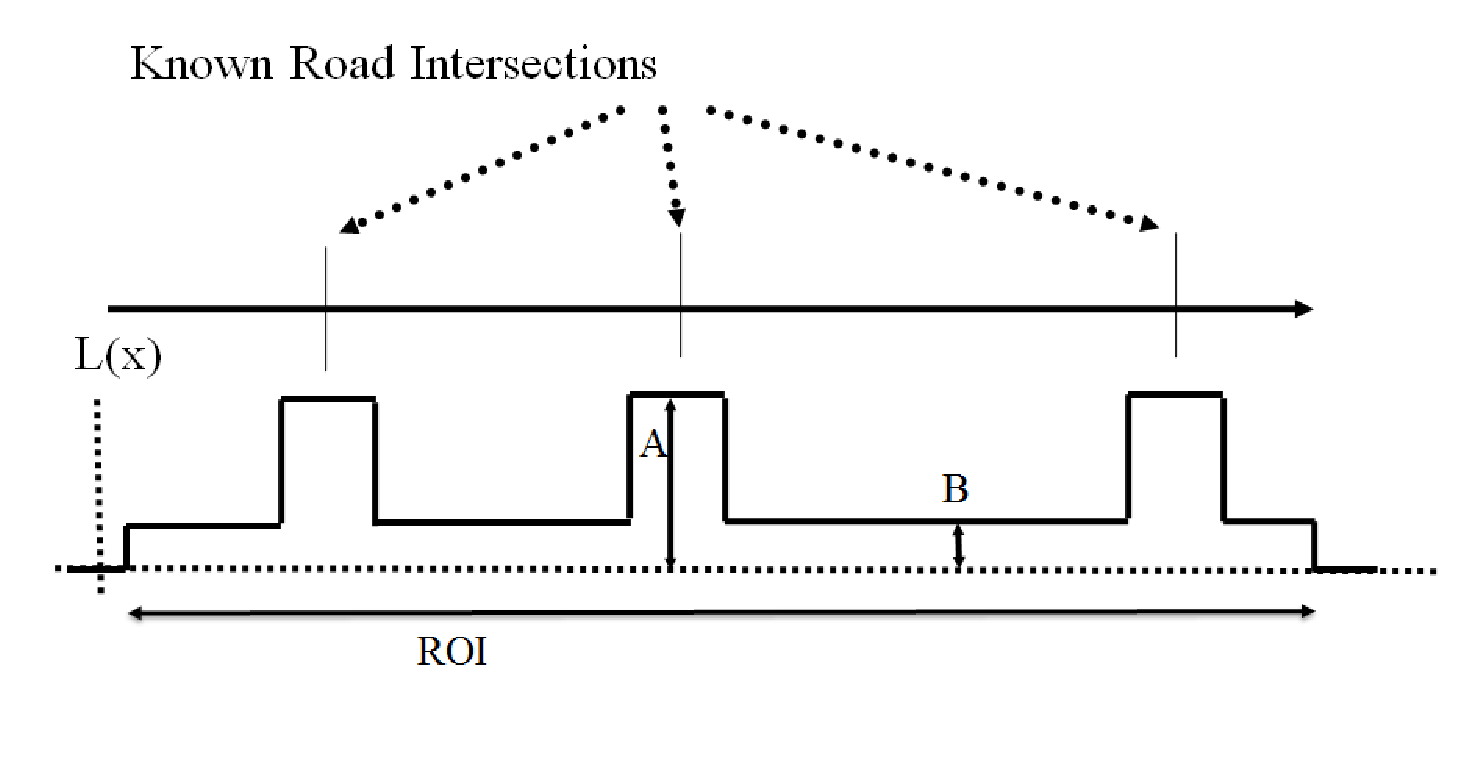
\includegraphics[width = 150mm]{Likelihood.eps}
    \caption{Likelihood $L(X)$ associated with the detection of a road intersection. $L(X)$ is equal to zero in any point outside the current ROI. Inside the ROI, it takes high values $(=A)$ at points that are close to known road intersections and low values $(= B,A\gg B>0)$ at points far from those known intersections.}
    \label{Fig::Likelihood}
\end{figure}

\section{Detection of Road Intersections Based on 3D Point Cloud}

Usually, there are diverse features that allow detecting a road intersection, such as traffic lights, pedestrian cross lanes, and also the pattern of the sites nearby. However, some of these characteristics may vary from cases of busy avenues to quiet neighborhood streets. Additionally, those are usually different in many countries as they have different rules and roads architecture. Therefore, techniques for inferring the proximity of road intersections should be based on some ``universally common'' feature, such as the boundaries of the roads themselves.

\subsection{Detection of Road Intersections}

The occupancy and re-emission grid map are used for detecting road intersections. But, a segmentation operation must be performed in the re-emission grid map (see Figure \ref{Fig::FIGURE_SEG_MAP1}) to highlight roads. For that, a simple threshold is used. To remove narrow regions of high re-emission (such as lane lines) the dilation morphological operation is employed. Figure \ref{Fig::FIGURE_SEG_MAP2} shows a typical result of our segmentation operation. This grip map is also used for the detection of road intersections and, from now on, we will call it simply filtered re-emission. 

\begin{figure}[t]
	\centering
	\subfloat[]{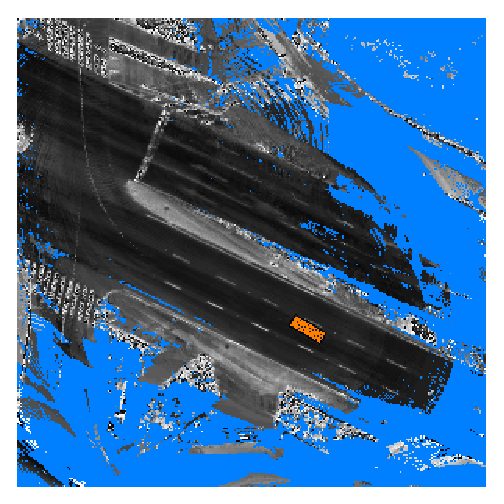
\includegraphics[width=42mm]{Remission1-1}
		\label{Fig::FIGURE_SEG_MAP1}}
	\subfloat[]{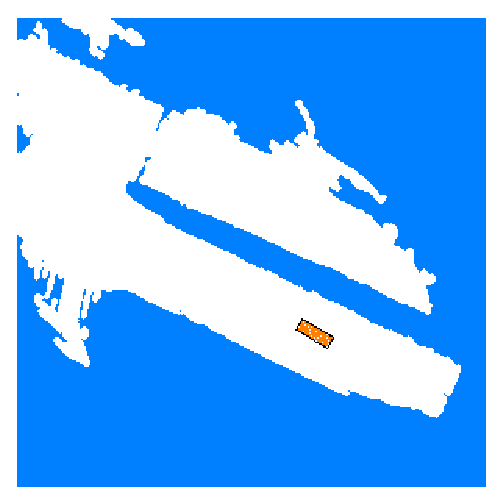
\includegraphics[width=42mm]{segmented2-1}
		\label{Fig::FIGURE_SEG_MAP2}}
	\caption{Filtered Re-emission map. (a) Re-emission grid map built by averaging the infrared reflectance of laser targets associated with each cell. The blue cells in (a) represent the parts of the environment that have not been scanned by the sensor. (b) Road-map extracted from (a) by thresholding and dilation. The white areas are classified as road surfaces, while the blue areas are classified as non-road surfaces.}
	\label{Fig::FIGURE_SEG_MAP}
\end{figure}

The detection process is based on the road width that we estimate using these grid maps. Given the grid maps (that represent the current surroundings of the vehicle) and the estimated position and orientation of the vehicle on these grid maps, exploration lines are generated from the lateral boundaries of the vehicle in its transversal direction (i.e. perpendicular to the longitudinal direction of movements of the vehicle). Each exploration line is used to find the first obstacle in the set of map cells crossed by it. This allows the estimation of the distance between a point at the border of the vehicle and the first obstacle (see Figure \ref{Fig::FIGURE_ROAD_SIZE} for an illustration of the concept).

\begin{figure}[t]
	\centering
	\subfloat[]{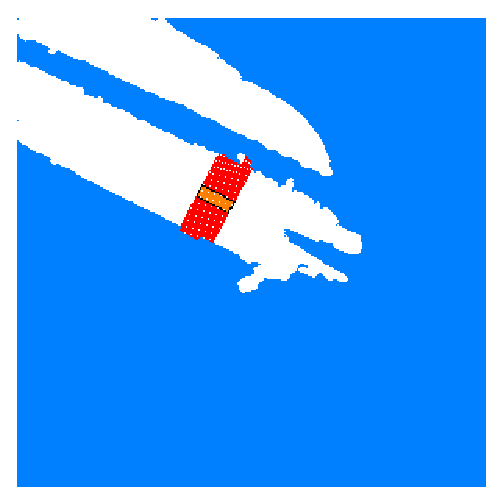
\includegraphics[width=42mm]{segmented1-2}
		\label{Fig::FIGURE_ROAD_SIZE1}}
	\subfloat[]{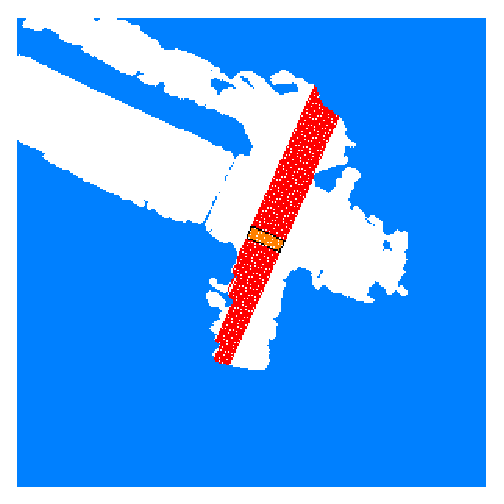
\includegraphics[width=42mm]{segmented1-1}
		\label{Fig::FIGURE_ROAD_SIZE2}}\\
	\subfloat[]{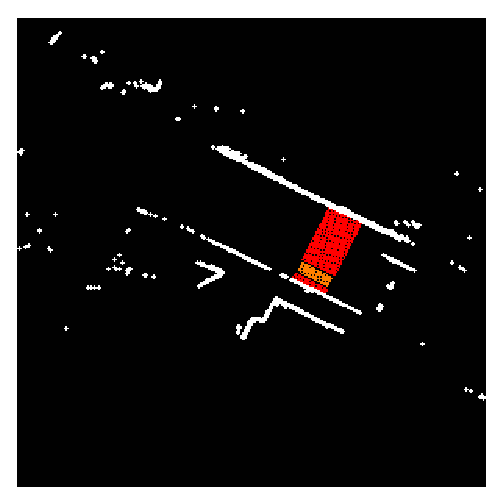
\includegraphics[width=42mm]{Occupancy2-1_black}
		\label{Fig::FIGURE_ROAD_SIZE3}}
	\subfloat[]{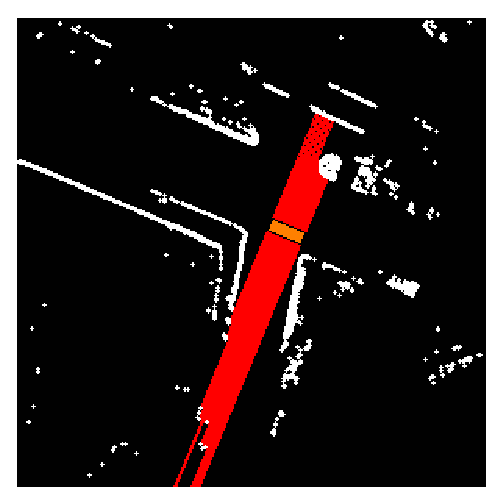
\includegraphics[width=42mm]{Occupancy2-2_black}
		\label{Fig::FIGURE_ROAD_SIZE4}}
	\caption{Transversal exploration lines. In red, the virtual scan performed by the transversal lines until they hit obstacles. The size of the lines is used to estimate the road width. The evolution of the estimated road width is used for inferring road intersections.}
	\label{Fig::FIGURE_ROAD_SIZE}
\end{figure}

This operation is performed on both sides of the vehicle. The pair of distances estimated for both sides allows estimating the width of the road. Each exploration line provides an instantaneous estimate of the road width, which is stored in a regressor. Exploration lines are not sampled by time but by space; consequently, the read width estimates are not affected by the speed of the vehicle.

Exploration lines are computed in both maps (occupancy grid map and filtered re-emission map), in order to mitigate the impact of the presence of other cars and imperfections in the filtered re-emission. The inferred width of the road is actually estimated as an average of the contents of the regressor (i.e., it is in fact a low pass filter). The use of these two maps is justified by the fact that they capture complementary information. In certain circumstances, the obstacle detection mechanism employed for building the occupancy grid  map cannot find any obstacle to infer the limits of the road, e.g. in cases of roads without curbs. However, in such cases, the re-emission information might still provide useful information to infer the boundaries of the road surface. In other situations, the re-emission information might be affected by traffic marks painted on the road surface, such as dense zebra crossing lines, but curbs might be present.

Even using both sources of information, there are cases when both are affected, e.g. when other cars (obstacles) are stopped nearby on the zebra lines during sufficient amount of time. Even in those cases, the inference process can avoid negative effects. Even though, in this context of application, the presence of false negatives (failure to infer a road intersection) is not crucial, while false positives (fictitious detection) would have a more negative impact. However false positives would still be tolerable by the localization process.

In order to reduce false negative during the intersection detection, the system does the correction by the intersection just when the particles are traveling close to one. To detect whether one particle is on a street junction or not, the same technique of exploration lines is applied for them in the road-map. As long as one particle is close to it, the system starts to evaluate the possibility of the car is on a road intersection. If the some particles have detected the intersection as well as the system, they will receive likelihood according to this, while the other ones the minimal likelihood. Consequently, during the particles resample the ones out of the intersection might be destroyed.




